\documentclass{article}

% if you need to pass options to natbib, use, e.g.:
% \PassOptionsToPackage{numbers, compress}{natbib}
% before loading nips_2016
%
% to avoid loading the natbib package, add option nonatbib:
% \usepackage[nonatbib]{nips_2016}

\PassOptionsToPackage{numbers,sort&compress}{natbib}
\usepackage{natbib}
\usepackage[final]{nips_2016} % produce camera-ready copy

\usepackage[utf8]{inputenc} % allow utf-8 input
\usepackage[T1]{fontenc}    % use 8-bit T1 fonts
\usepackage{hyperref}       % hyperlinks
\usepackage{url}            % simple URL typesetting
\usepackage{booktabs}       % professional-quality tables
\usepackage{amsfonts}       % blackboard math symbols
\usepackage{nicefrac}       % compact symbols for 1/2, etc.
\usepackage{microtype}      % microtypography
\usepackage{graphicx}
\usepackage{subcaption}
\usepackage{csquotes}
\usepackage{amsmath}
\usepackage{amssymb}
\usepackage{array}
\usepackage{makecell}
\usepackage{float}
\usepackage{multirow}
\usepackage{pdfpages} 

\newcommand{\minisection}[1]{\textbf{#1}\quad}

\title{Genre Prediction and Music Recommendation}

% The \author macro works with any number of authors. There are two
% commands used to separate the names and addresses of multiple
% authors: \And and \AND.
%
% Using \And between authors leaves it to LaTeX to determine where to
% break the lines. Using \AND forces a line break at that point. So,
% if LaTeX puts 3 of 4 authors names on the first line, and the last
% on the second line, try using \AND instead of \And before the third
% author name.

\author{
  s2202209\\
  %% examples of more authors
  \And
  s2176992\\
 \And
  s2185011\\
  \And
  s2188036
}

\begin{document}

\maketitle

\begin{abstract}
This paper explores the tasks of single-genre classification and content-based song recommendation on Spotify's Top 200 playlists from 2017-2023. Using supplementary track-level data, we built models to predict `super-genres' given a track's features, finding a random forest model performs best across accuracy, ROC-AUC, Macro-F1, and MCC. We then built a content-based song recommender using both audio features and lyric-based semantic and TF-IDF embeddings, evaluating via clustering metrics. Lyric semantic embeddings result in the best recommendation performance, with hybrid models performing approximately on par when genre information is included.

\end{abstract}




\section{Introduction}
\vspace{-3mm}
%\begin{itemize}
%\item Introduction
Streaming has forever altered the landscape of the music industry, with easy access to hundreds of millions of songs leaving consumers overwhelmed by choice. Recommender systems that leverage machine learning algorithms have thus become commonplace in music streaming platforms to help narrow the search for new music, finding tracks consumers find relevant and engaging. Genre information plays a key role in this search, as it implicitly organises broad swathes of music into related clusters, increasing the likelihood of finding relevant music.  The task of automatically inferring genre from track-level features is thus especially critical within music recommendation systems. 

Genres are inherently ambiguous as they are human-assigned and not derived through objective track features. Furthermore, tracks may have multiple genres, which increases the problem space of classification. In this paper, we focus on the single-genre classification task. Similarly, recommendation systems are difficult to evaluate, as a recommendation may be correct for some, and incorrect for others. To simplify the problem, we define concrete performance metrics which allow for direct comparison between models.

Previous work on genre classification has used independent recurrent neural networks (IndRNNs), pre-trained convolutional neural networks, and traditional machine learning methods (logistic regression, K-nearest neighbours). \citet{wu2018music} argue that machine learning performance depends heavily on the quality of feature extraction, so opt for an IndRNN. \citet{kumar2016comparative} found that neural networks were most adept at single-genre classification task compared to traditional methods. Finally, \citet{ru2023improving} extend to multi-genre classification, combining audio and lyrical features to achieve state-of-the-art performance on the Music4All dataset, confirming the effectiveness of combining audio and lyrical features. 

Recent track recommendation systems tend to focus on collaborative filtering methods, deep learning approaches, and content-based recommendation \citep{7910613, schedl2019deep, soleymani2015content}. Given the lack of user listening history and computational constraints, collaborative filtering and deep learning methods are deemed infeasible for this report. We thus chose to focus on building a content-based recommender, that makes meaningful suggestions based on track-level and supplementary features.

In this report, we use the Spotify Top-200 dataset for two tasks: weakly supervised genre classification, and content-based track recommendation. We consider genre classification to be weakly supervised because track genres are inferred from Spotify artist genres, which are incomplete. We first apply exploratory data analysis methods on the dataset, including PCA and correlation heatmaps, before utilising external APIs to enhance the feature set of the data. With our enhanced dataset, we clean the data and normalise, before comparing several machine learning methods at the genre classification task. Additionally, we incorporate the predicted genres into a track recommender, comparing performance with and without genre included.

\vspace{-3mm}
\section{Data Preparation}
\vspace{-3mm}
\minisection{Description of Dataset} The original dataset consists of Spotify's `Top 200' playlists collected from across the globe, from January 2017 to May 2023. It includes 651,936 rows, each of which corresponds to the appearance of that song within the `Top 200' playlist for a given day. Entries contain metadata about the song (e.g. Title, Date, Song URL) and data about the artist (e.g. Nationality, Continent). We utilise the additional track audio features provided by the User-engagement and Metrics team (e.g. energy, danceability, acousticness) to aid our exploration of the data.

\minisection{Data Cleaning} Initial inspection of the data highlighted several aspects of the data that required cleaning. We note: \textbf{(1)} entries were duplicated depending on the number of artists (one for each artist), differing only by artist metadata and split of assigned points. \textbf{(2)} The `Loudness' feature appears to be improperly scaled. 

To address duplicate entries, we consolidate rows by creating `Primary Artists' and `Featuring Artists' columns, extracted via regex expressions on song titles, resulting in a reduced 467,070 entries. To rescale `Loudness', we assume the values of `Loudness' correspond to dBFS (Decibels relative to Full Scale), which for digital audio typically fall into a range of [-22 (very quiet) to 0 (maximum loudness)]. A histogram of the original `Loudness' values (shown in Appendix \ref{appendix:loudness}) revealed values were heavily skewed to a range of [-20000,-2500], with a small subset appearing to reflect the likely correct dBFS values. We rescale the majority of skewed values by a factor of 1,000, and manually adjust three entries with positive `Loudness' values.

\minisection{Dropped Features} Due to the nature of our chosen tasks, we drop any temporallly related features, namely: Date, Rank, and Points (Total). The dataset without temporal data allows us to explore the underlying relations between songs, artists, and their features.

\minisection{Feature Enrichment} Next, we enrich our dataset with the following additional features from the Genius \footnote{\url{https://docs.genius.com/}} and Spotify \footnote{\url{https://developer.spotify.com/documentation/web-api/}} APIs: \texttt{lyrics, artist\_id, explicit, track\_popularity, artist\_followers, artist\_genres, artist\_popularity}. Of the 9,161 unique tracks, lyrics were obtained for 8,034 songs. Additionally, we utilise the \texttt{lingua-py} Python library to extract the language(s) of each song, adding the following features \texttt{detected\_languages, num\_languages, language\_confidences}. Next, to perform PCA on our pre-processed dataset, we one-hot encode the \texttt{detected\_languages, continent, nationality} features in our non-temporal dataset. This results in 131 features for 9,161 unique songs. 

\minisection{`Super-Genre' Mapping} The original dataset contains no genre feature. We utilised the Spotify API to extract genres associated with the artist of each song, resulting in 346 unique sub-genres, from psychedelic rock to emo rap. A limitation of the Spotify API is that genres were not returned for all artists. Figure \ref{fig:supergenres} shows the distribution of genres among songs for which the Spotify API did not return a genre. Out of all unique tracks, 5,271 were assigned a super-genre, leaving 3890 tracks with no genre. To simplify the scope of the task, we determined a list of `super-genres' to map existing sub-genres into, shown in Figure \ref{fig:super-genres}. The `other' super-genre contains those genres which do not easily fall into the previously defined super-genres. These include: \texttt{["christmas", "comedy", "hollands"]}. Some songs, e.g. Carol of the Bells by John Williams, were considered to be in the `other' genre (in this case `performance') by our assumption that song genre equates to artist genre. As genre is inherently subjective and we consider only single-genre classification, we consider this to be a necessary (and acceptable) ambiguity.

To perform the mapping of sub to super-genre, we initially applied agglomerative clustering. The resulting clusters were either nonsensical, or resulted in completely empty clusters, so this method was discarded. Instead, we chose to manually annotate the music into the following designated super-genres: rap, pop, electronic, hip hop, dance, trap, rock, folk, r\&b, country, metal, funk, indie, jazz, soul, alternative, religious, performance and other.

\vspace{-3mm}
\section{Exploratory Data Analysis}
\vspace{-3mm}
\minisection{Correlation Heatmap} To gain an insight into surface-level connections between our numerical features, we produce a correlation heatmap, shown in Figure \ref{fig:corrHeatmap}. Certain obvious correlations appear, such as `Valence' and `Energy' (positive), and `Energy' and `Acousticness' (negative). As the heatmap shows, there are no surprising correlations in the data, we turn to further exploratory data analysis methods for insight.

\begin{figure}[!h]
  \centering
  \begin{minipage}{0.48\textwidth}
    \centering
    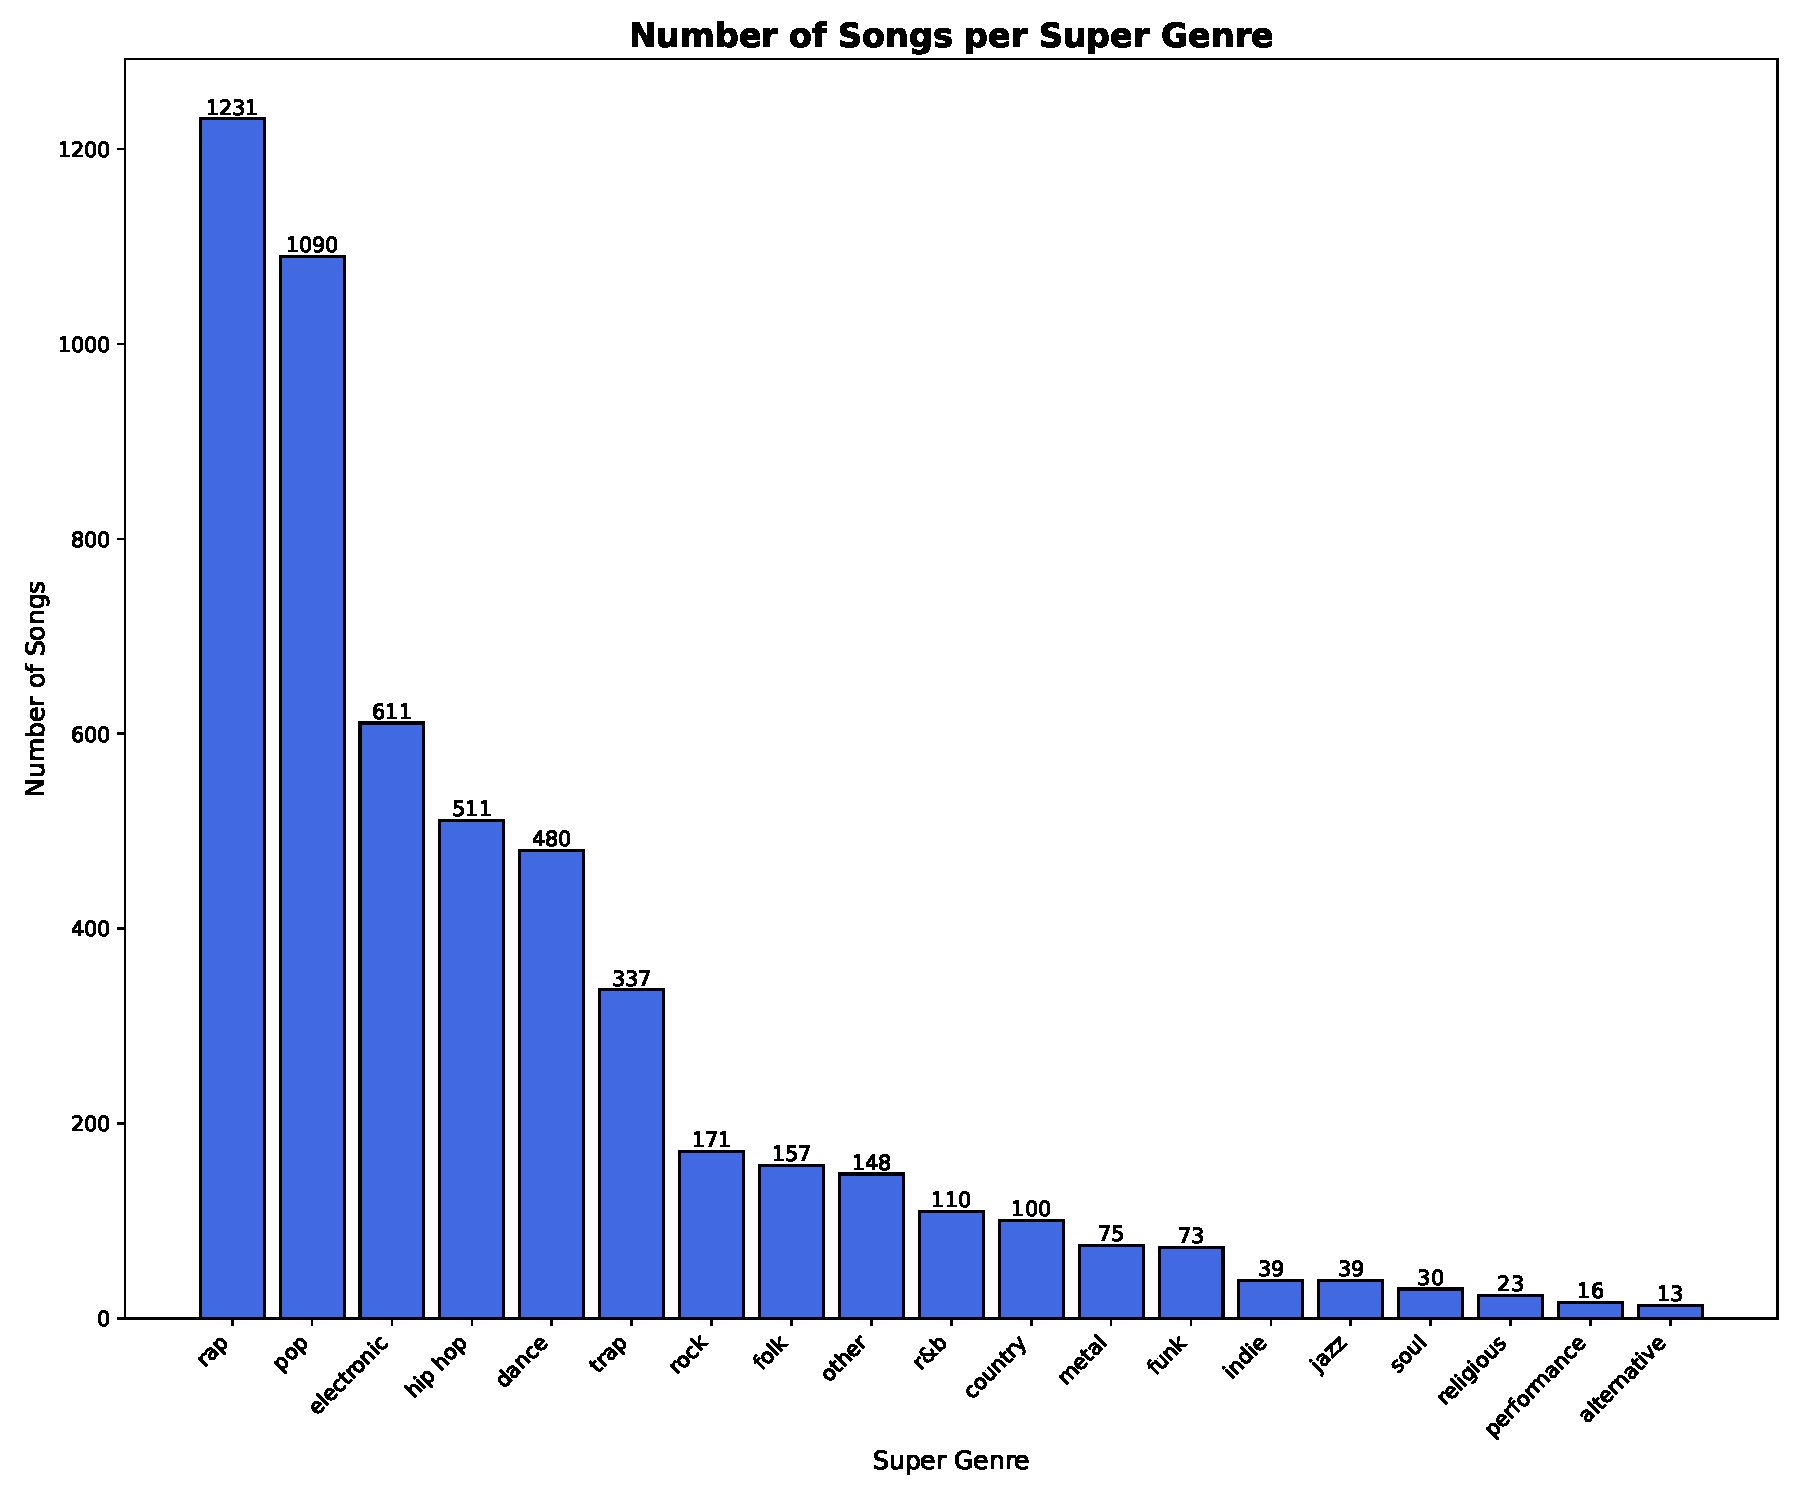
\includegraphics[width=\textwidth]{images/songsSuperGenre.pdf}
    \caption{Super-genre distribution histogram}
    \label{fig:supergenres}
  \end{minipage}\hfill
  \begin{minipage}{0.48\textwidth}
    \centering
    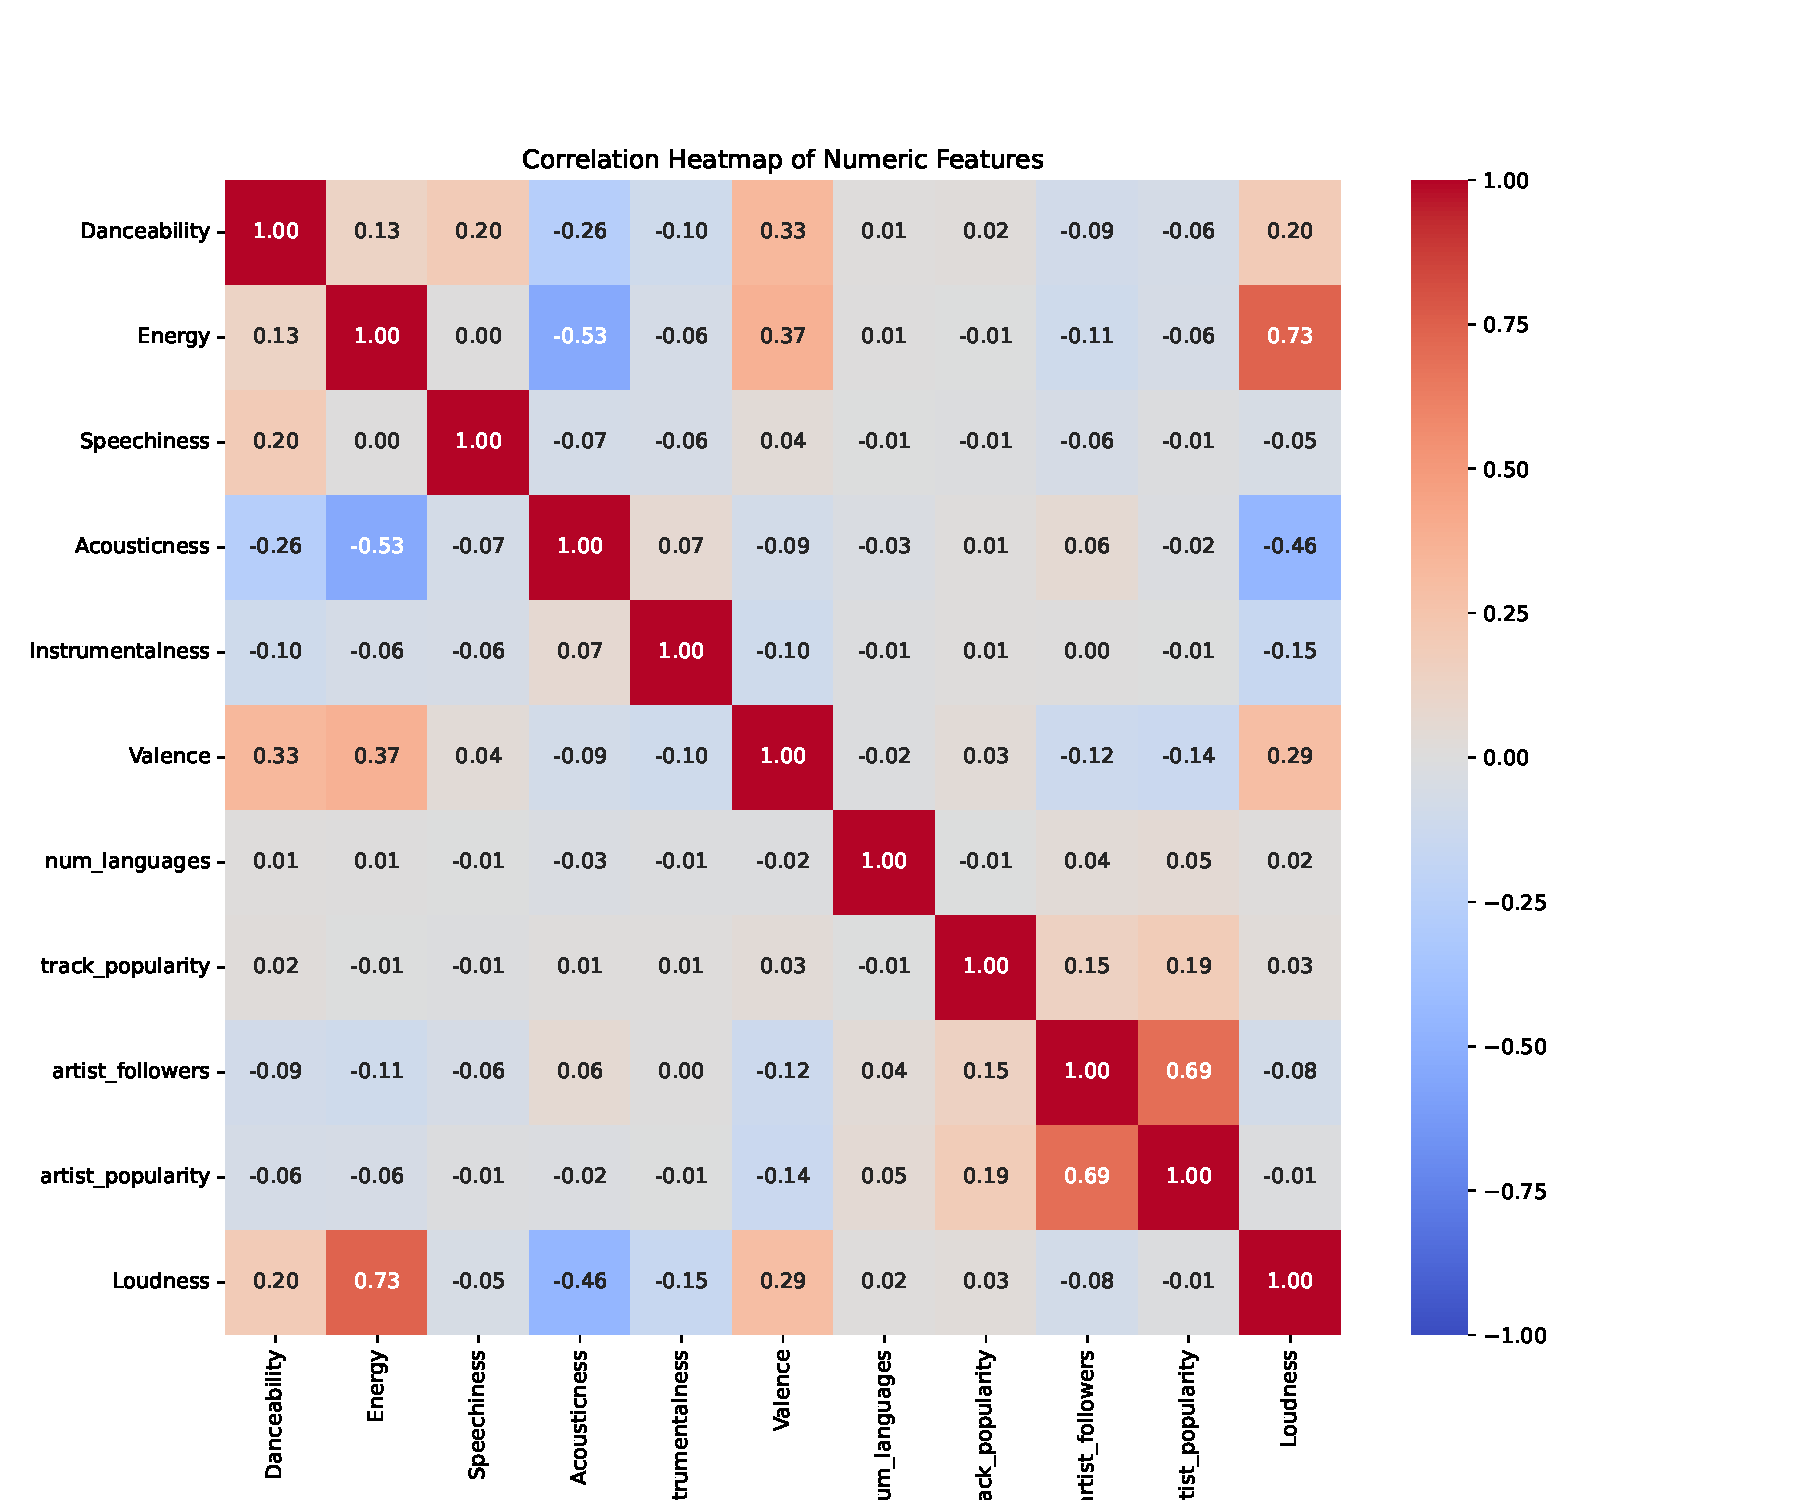
\includegraphics[width=\textwidth]{images/Correlation_heatmap.pdf}
    \caption{Cleaned Features Correlation Heatmap}
    \label{fig:corrHeatmap}
  \end{minipage}
\end{figure}




\minisection{Principal Component Analysis} In order to extract meaningful insights from our newly enriched dataset, we perform PCA on the seven audio features, along with one-hot encodings for nationality, continent, and language. We normalise our data prior to performing PCA. We visualise the first and second principal components in Figure \ref{fig:PCA}. From the visualisation, we can see that there is clear clustering around certain directions of the principal component space. However, due to the relatively small number of features than is typical to use with PCA, out of 131 original features, 95\% of the variance is explained by 98 features. This indicates that while the first two principal components provide an interesting visualisation of the data, a much more complex model is required to capture the majority of the datasets variance. 

\begin{figure}[h]
\centering
\begin{minipage}{0.48\textwidth}
    \centering
    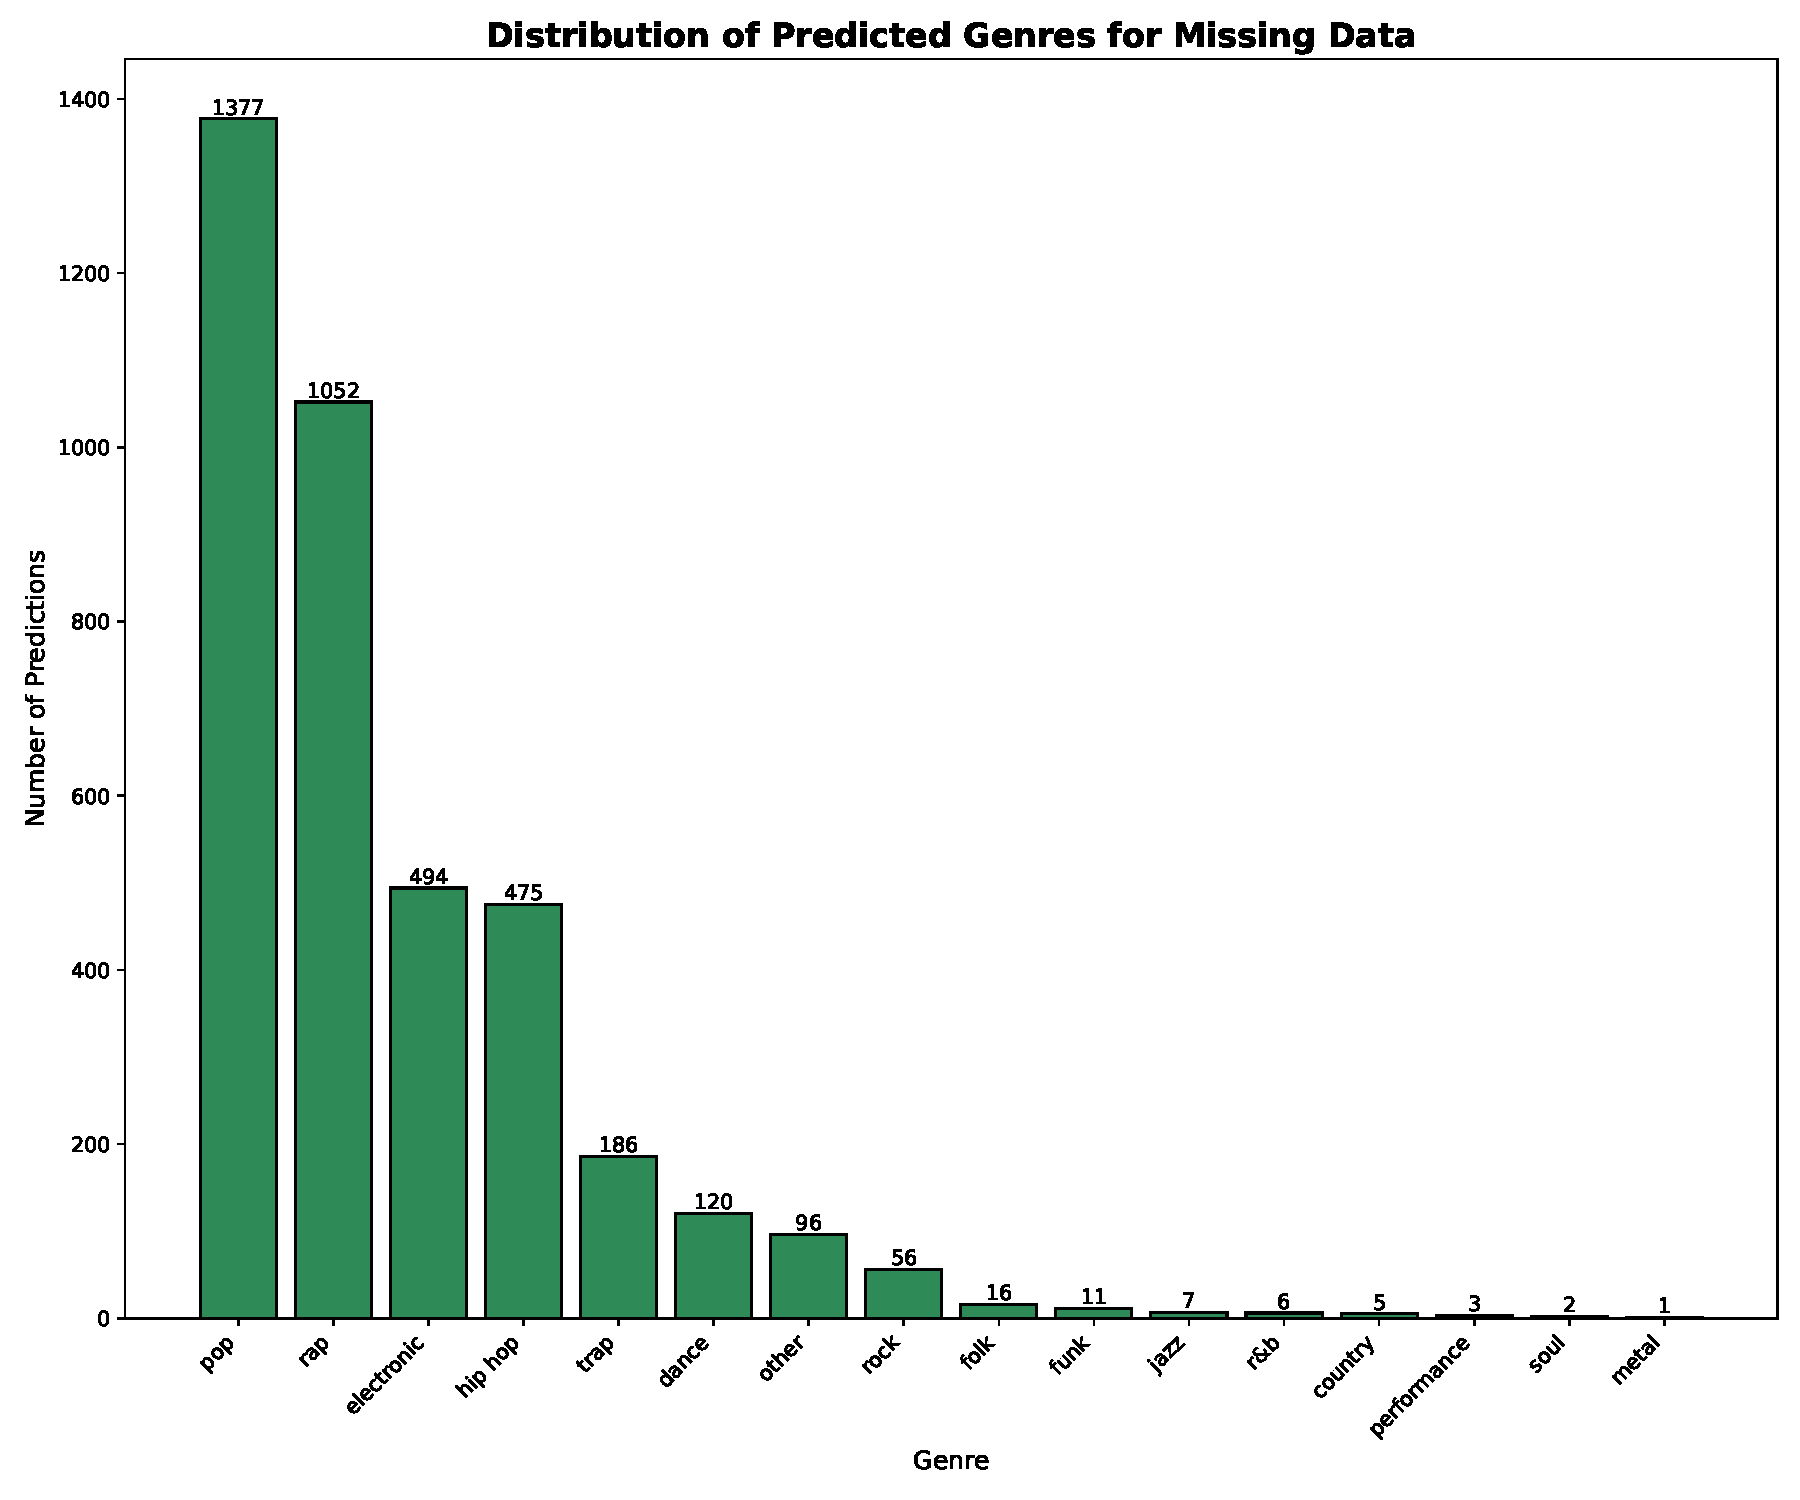
\includegraphics[width=\textwidth]{images/genres_distribution_missing_data.pdf}
    \caption{Distribution of genres from the Random Forest Model}
    \label{fig:genres_distribution_missing_data}
\end{minipage}
\hfill
\begin{minipage}{0.48\textwidth}
    \centering
    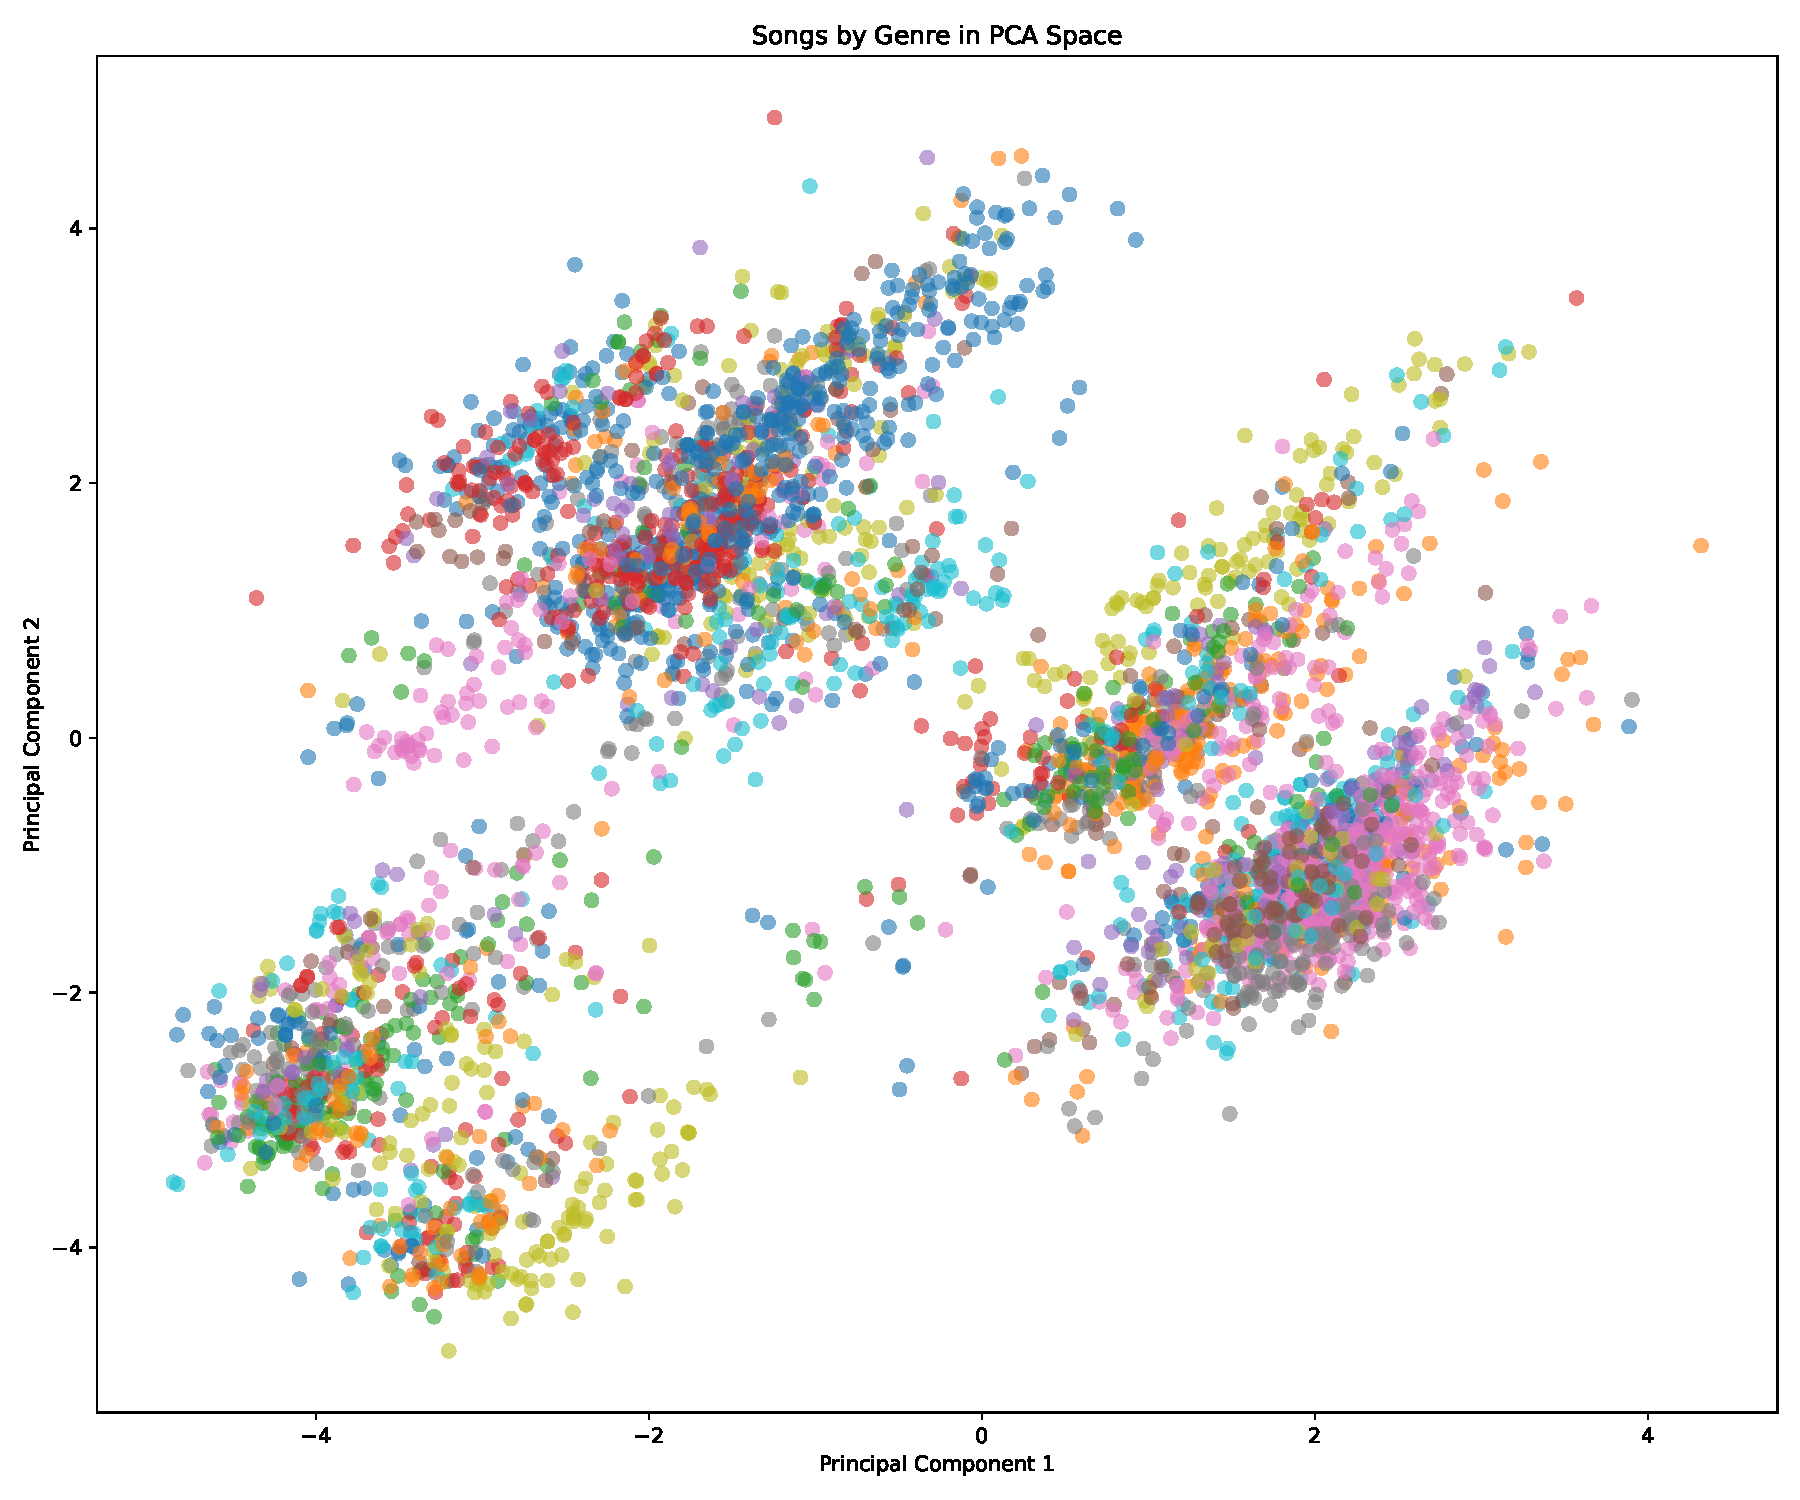
\includegraphics[width=\textwidth]{images/pca.pdf}
    \caption{PCA visualisation of the first two principal components}
    \label{fig:PCA}
\end{minipage}
\end{figure}

\vspace{-3mm}
\section{Primary Task: Genre Prediction}\label{task:genre-prediction}
\vspace{-3mm}
\minisection{Methodology} We train our models on the 5,271 songs with genre labels to predict genres for the remaining 3,890 songs, which we later use for our recommender system. We assume that a track's genre aligns with its artist's primary genre, and is therefore used as a reliable proxy. It was crucial to predict the genre for the unlabelled songs, as this data was going to be used for our Song Recommender System (See Section \ref{task:song-recommendation}). We implemented four different types of models: Logistic Regression, Decision Tree, Random Forest Classifier, and a Neural Network. We filtered the dataset to include only tracks with a genre label, then split it into training (60\%), validation (20\%), and test (20\%) sets \cite{AI_2025}.

Given the imbalanced nature of our labelled dataset, accuracy becomes an unreliable measure for assessing performance \cite{Brownlee_2021}. We thus utilise additional evaluation metrics such as ROC-AUC (Receiver Operating Characteristic Area Under the Curve), Log Loss, F1-Macro and Matthews Correlation Coefficient (MCC). The ROC-AUC score tells us how effective the classifier is in differentiating between the positive and negative classes. Log Loss penalises models more severely for making wrong predictions confidently, so this takes into account the “uncertainty of predictions” \cite{AI_2024}. F1-Macro takes an unweighted average of per-class F1 scores, giving all genres equal importance regardless of their frequency, making it an appropriate metric given the nature of our dataset \cite{Sefidian_2024}. The MCC is suitable for imbalanced data as provides a balanced measure of the quality of the classification \cite{learn_2025}. 


\minisection{Evaluation} To establish a minimum performance expectation, we implemented a baseline model which always predicts the genre ‘pop’, as our other models assign `pop' most commonly. For ROC-AUC, a score of 1 indicates a perfect classification model, whereas a random model would have an AUC of 0.5 \cite{AI_2025a}. Our baseline model outputted a ROC-AUC score of 0.5 (See Table \ref{tab:model_comparison}), proving it an effective baseline model.

For our second model, we implemented a multinomial logistic regression model, resulting in an ROC-AUC score of 0.84 on the validation set. Since our data was imbalanced, the variable \texttt{class\_weight} with the value \texttt{balanced} takes class frequency into account and adjusts the weight accordingly for each class. This resulted in an ROC-AUC score of 0.85. Additionally, we tuned the hyperparameter \texttt{max\_iters} and found the optimal value of 900 iterations resulted in the highest ROC-AUC score, and thus was selected for our final model (see Appendix \ref{appendix:genre-classifications} Table \ref{tab:max_iter_results}).

For the decision tree, \texttt{max\_depth} defines the tree’s maximum depth, and \texttt{min\_samples\_leaf} sets the minimum number of samples needed for a node to become a leaf. If either is too low or too high, this can result in over/underfitting of the data \cite{forGeeks_2025}\cite{Hankare_2023}. We tuned these parameters to maximise ROC-AUC, achieving the best score of 0.859 with \texttt{max\_depth=7} and \texttt{min\_samples\_leaf=20}, a slight improvement from the Logistic Regression Model(See Table \ref{tab:hyperparameter_tuning}). 

We implemented a multi-layer feedforward neural network, with three dense layers, and a softmax output with 19 outputs (one per super-genre). We use categorical cross-entropy, implementing early stopping on validation loss with learning rate reduction, and a batch size of 64 training over 200 epochs. The training goal was to optimise ROC-AUC on the validation set, resulting in an ROC-AUC of 0.898 on the test set. Exact hyper-parameters can be found in Appendix \ref{appendix:genre-classifications} Figure \ref{tab:hyperparam}.

Our random forest model achieved an ROC-AUC score of 0.937, outperforming all previous models. The \texttt{n\_estimators} parameter determines the number of trees which can improve model performance \cite{Shafi_2025}. We tuned \texttt{max\_depth} , \texttt{n\_estimators} and \texttt{min\_samples\_leaf} , obtaining an ROC-AUC 0.943 with \texttt{max\_depth =20, min\_samples\_leaf = 1, n\_estimators = 160}. (See Appendix \ref{appendix:genre-classifications} figures \ref{fig:max_depth}, \ref{fig:min_samples_leaf}))



\begin{table}[h]
\centering
\caption{Model Performance Comparison}
\label{tab:model_comparison}
\begin{tabular}{lccccc}
\hline
\textbf{Model} & \textbf{Accuracy} & \textbf{ROC AUC} & \textbf{Log Loss} & \textbf{F1-Macro} & \textbf{Matthews Corrcoef} \\
\hline
Baseline (Always Pop) & 0.2036 & 0.5000 & 28.7046 & 0.0178 & 0.0000 \\
Logistic Regression & 0.3473 & 0.8370 & 2.1399 & 0.2639 & 0.2871 \\
Decision Tree & 0.4976 & 0.8689 & 2.6534 & 0.2420 & 0.4141 \\
Random Forest & \textbf{0.6955} & \textbf{0.9344} & \textbf{1.2177} & \textbf{0.5675} & \textbf{0.6463} \\
Neural Network & 0.5176 & 0.898 & 1.4917 & 0.2973 & 0.4358 \\
\hline
\end{tabular}
\end{table}

As seen in table \ref{tab:model_comparison}, all models outperform the baseline model. We note that generally accuracy is quite low (<50\%), but it is highest for the Random Forest Model. The log loss is extremely low for the random forest model, indicating its confidence in its predictions, which makes it a reliable model. Across all metrics, the Random Forest Model outperforms other models.

With our Random Forest Model we now predict the genres for the tracks with missing genres. The class distribution of our predicted genres follows closely the original set of labelled genres (see Figure \ref{fig:genres_distribution_missing_data}), indicating the model doesn't introduce a significant bias toward any particular genre, including the most common ones.


\minisection{Limitations} Our data was not a completely balanced representation of songs from all the different genres, which can bias our model towards the majority classes. We also manually categorised subgenres into super-genres through research and listening to music samples, acknowledging that this classification involves inherent subjectivity. The decisions were made by our small team, which may not represent a broader consensus given how genres can overlap. For a more confident classification, a larger group of annotators with established inter-annotator agreement would be robust. 

\vspace{-3mm}
\section{Secondary Task: Song Recommendation}\label{task:song-recommendation}
\vspace{-3mm}
The key issue most recommendation systems run into is the subjectivity of taste. Suppose a user particularly likes \enquote{No Time to Die} by Billie Eilish; would another Billie Eilish song be a good suggestion? How is the system to account for the fact that our user just really likes Daniel Craig era James Bond? To build a recommendation system without data giving explicit relations between songs (e.g. playlists and albums) we must make some basic assumptions, from which we can make quantitative statements about the relative quality of recommendations.

The first assumption we make is that in the above case, recommending another Billie Eilish song is a good recommendation. If we assume that songs by the same artist are good recommendations, we can use the fact a model recommends these songs as a proxy for the relatedness of its other recommendations. We make the same assumption when recommending songs within the same genre.

\minisection{Methodology} We built four models and compared them with random predictions against five metrics. Each model constructs an embedding space and performs KNN to make predictions. Our base model `features' uses only the seven audio features, `TF-IDF' and `semantic' expand on this with word usage similarity and semantic similarity in lyrics respectively. The `hybrid' model blends between TF-IDF and semantic. Each model also had a version with one-hot encoded genre data. We use the following metrics: `silhouette score' to measure cluster quality, `mean pairwise distance' to measure how diverse songs are in the dataset, and `embedding efficiency' given by $\frac{\text{silhouette}}{\text{variance}}$ to determine if the model is dominated by noise. We also have two coherence scores, which measure how well songs by the same artist or from the same genre get clustered together.

The embedding spaces for the hybrid model were constructed by weighting the TF-IDF and semantic components. The final embedding is created by normalising the embedding given by either component and taking a weighted sum. If their dimensions differ then zero padding is used. The best hybrid is then determined by parameter sweep in intervals of $10\%$ between $0\%$ and $100\%$ semantic, with the winner being the highest scoring model by the following metric: $$\text{score} = 0.4 \times \text{silhouette score} + 0.3 \times (\text{artist coherence} + \text{genre coherence})$$
All models were tested three times on encodings built from the 8,034 songs in the dataset with lyrics: once with no genre data, once with one-hot encoded genre data with an `other' category (i.e. no predicted genres), and once with genres predicted by the random forest model described in Section \ref{task:genre-prediction}. Results are shown in Tables \ref{tab:prediction-clustering-base}--\ref{tab:prediction-clustering-random-forest}, where the best hybrid model blend is displayed as a ratio between TF-IDF and semantic, e.g. (40:60) for 40\% TF-IDF and 60\% semantic.
\begin{table}[h!]
\centering
\footnotesize
\begin{tabular}{l|cccccc}
\textbf{Metric} & \textbf{Features} & \textbf{TF-IDF} & \textbf{Semantic} & \textbf{Hybrid (50:50)} & \textbf{Random} & \textbf{Best} \\
\hline
Silhouette Score               & $\mathbf{0.1654}$ & $0.0151$ & $0.0617$ & $0.0161$ & $0.0066$ & Features \\
Mean Pairwise Distance         & $0.9862$ & $0.9680$ & $\mathbf{0.6725}$ & $0.9680$ & $1.0000$ & Semantic \\
Embedding Efficiency           & $0.0236$ & $0.0156$ & $\mathbf{0.0918}$ & $0.0167$ & $0.0001$ & Semantic \\
Artist Coherence Score         & $0.1991$ & $0.0686$ & $\mathbf{0.4383}$ & $0.0686$ & $0.0003$ & Semantic \\
Genre Coherence Score          & $0.2209$ & $0.0583$ & $\mathbf{0.4113}$ & $0.0583$ & $0.0001$ & Semantic \\
\end{tabular}
\vspace{0.25em}
\caption{Clustering performance across embedding types w/o genre}
\label{tab:prediction-clustering-base}
\centering
\footnotesize
\begin{tabular}{l|cccccc}
\textbf{Metric} & \textbf{Features} & \textbf{TF-IDF} & \textbf{Semantic} & \textbf{Hybrid (50:50)} & \textbf{Random} & \textbf{Best} \\
\hline
Silhouette Score           & $0.1294$ & $0.2766$ & $\mathbf{0.3225}$ & $0.2132$ & $0.0067$ & Semantic \\
Mean Pairwise Distance     & $0.9492$ & $0.8703$ & $\mathbf{0.7226}$ & $0.8378$ & $0.9977$ & Semantic \\
Embedding Efficiency       & $0.0166$ & $0.1590$ & $\mathbf{0.2232}$ & $0.0848$ & $0.0001$ & Semantic \\
Artist Coherence Score     & $0.3545$ & $0.5350$ & $\mathbf{0.7156}$ & $0.6900$ & $0.0101$ & Semantic \\
Genre Coherence Score      & $0.3592$ & $0.5292$ & $\mathbf{0.7056}$ & $0.6862$ & $0.0101$ & Semantic \\
\end{tabular}
\vspace{0.25em}
\caption{Clustering performance w/ one-hot genres (missing values)}
\label{tab:prediction-clustering-one-hot}
\begin{tabular}{l|cccccc}
\textbf{Metric} & \textbf{Features} & \textbf{TF-IDF} & \textbf{Semantic} & \textbf{Hybrid (40:60)} & \textbf{Random} & \textbf{Best} \\
\hline
Silhouette Score               & $0.1284$ & $0.2470$ & $0.2825$ & $\mathbf{0.4060}$ & $0.0067$ & Hybrid \\
Mean Pairwise Distance         & $0.9591$ & $0.8978$ & $\mathbf{0.7500}$ & $0.8744$ & $0.9982$ & Semantic \\
Embedding Efficiency           & $0.0164$ & $0.1376$ & $\mathbf{0.1883}$ & $0.1548$ & $0.0001$ & Semantic \\
Artist Coherence Score         & $0.3439$ & $0.4933$ & $\mathbf{0.6423}$ & $0.6018$ & $0.0088$ & Semantic \\
Genre Coherence Score          & $0.3522$ & $0.5240$ & $\mathbf{0.6927}$ & $0.6826$ & $0.0100$ & Semantic \\
\end{tabular}
\vspace{0.25em}
\caption{Clustering performance w/ random forest prediction for missing genres}
\label{tab:prediction-clustering-random-forest}
\end{table}

\minisection{Evaluation} Predictably, all models performed substantially better than the random baseline in all cases. The feature-only models performed poorly, but improved with the inclusion of genre data. Adding encoded lyrical similarity helped the models significantly, though TF-IDF in the genre-less case made the features model worse. This suggests that similar phrasings are useful in prediction, but only within genres. The semantic embeddings performed best of all the models, with the genre-less semantic model being the only one to get a pair-wise difference significantly better than the random encoding. Given the relative underperformance of TF-IDF, the hybrid model is largely worse than the semantic one. The improved silhouette score with random forest predicted genres suggests that the model is creating more clearly divided distinctions between song clusters, and the relatively similar embedding efficiency suggests that this is not merely noise, however the semantic model outperforms in terms of pairwise distance and the coherence scores and is therefore still favourable. The effect of one-hot genre encodings on our results matches results from the literature, which suggest that genre is the single most important feature for song prediction \citep{abhilash2020identifying}.

We note that the results with missing genres are slightly better (except pairwise distance) than those with fully annotated genres. It seems likely that this is due to a disconnect between our genre annotations and our assumption about artist genre corresponding to song genres. Where our assumption suggests every John Williams song is a performance --- e.g. `Carol of the Bells' --- our classifier instead predicts it would be a jazz song (see Figure \ref{fig:carol} in Appendix \ref{appendix:genre-classifications}).

From a subjective standpoint, the recommendations produced are coherent, if excentric in cases. The dataset is not representative of many kinds of music and so struggles for artists in non-pop, non-rap genres (as we'd expect from Figure \ref{fig:supergenres}), though the models considering lyrical similarity accurately collect certain kinds of music together well. For instance Christmas music is clustered very well even when these songs have differing genres, see Table \ref{tab:carol-of-the-bells} in Appendix \ref{appendix:recommendations}.

\minisection{Limitations} Our models are limited by our dataset. Were we to have data about more than just songs, e.g. playlist, album, and user data, we could have applied more sophisticated techniques like collaborative filtering and considered more of the context in which any given song is listened to (`sad' playlists, film soundtracks with many artists, etc.) when giving recommendations, similar to the methods applied in state of the art models like those used by Spotify itself \citep{Wong_2024}. We also recognise that our dataset is heavily skewed in terms of genre representation as mentioned, meaning that our recommendation quality for music which isn't in the highly represented genres is limited. We are confident, however, that given a more complete dataset our approach would generalise well.

\vspace{-3mm}
\section{Conclusion}
\vspace{-3mm}
This report evaluates the effectiveness of machine learning techniques for the tasks of single-genre track classification, and content-based song recommendation. For genre classification, we found that a random forst model outperforms logistic regression, decision trees, and a neural network (accuracy=0.696, MCC=0.65, macro-F1=0.57, ROC-AUC=0.93). For song recommendation, lyric semantic embeddings result in the strongest clustering coherence, with our hybrid TF-IDF-semantic performing similarly with included genre information. Certain limitations remain for both tasks. For genre classification, we assume a tracks' genre is the most common genre of the artist. In reality, songs can have more than one genre and those genres may be new for the artist. Future work could focus on multi-genre classification, or hand annotating a small subset of the overall tracks for a more accurate initial genre assignment. For our song recommender, we were limited by the diversity of the data in terms of genre, and had no data linking songs explicitly with which to evaluate recommendations. Future work could expand the dataset beyond the most popular tracks to be more representative, and use connective data like personal playlists and albums. This would allow for collaborative filtering, which requires making fewer and better founded assumptions about what makes for a quality recommendation.

\newpage
\section{Statement of Contributions}
\begin{itemize}
    \item s2176992
    \begin{itemize}
        \item participated in many of our initial brainstorming sessions and came up with many ideas to investigate. Such as, investigating the effect of featuring artists have on the success of songs in terms of their lifetime in the top 200 playlists.
        \item Helped with the manual verification of the cleaning of our dataset.
        \item prepared the dataset for Principal Component Analysis by one-hot encoding the categorical information, and also carried out PCA
        \item researched, implemented and hypertuned Random Forest Classifier models for our genre prediction task, and evaluated its performance compared to the other models. 
        \item tried to apply agglomerative clustering to map the sub genres to super genres which was unsuccessful so they organised the 346 genres into 19 genre super classes manually
        \item helped write the section 4: Genre Prediction
    \end{itemize}
    \item s2202209
    \begin{itemize}
        \item also tried agglomerative clustering, and helped organise the sub genres into super genres
        \item helped enrich the dataset by adding additional features using the Genius and Spotify APIs.
        \item used the python library \texttt{lingua-py} to get the language(s) for each track which added more features
        \item implemented, hypertuned and evaluated the Logistic Regression, Decision Tree and Baseline model.
        \item helped write the section 4: Genre Prediction
    \end{itemize}
    \item s2185011
    \begin{itemize}
        \item Wrote the abstract, introduction, data preparation, and conclusion sections
        \item Implemented, tuned, and evaluated the neural network for the genre prediction task
        \item Cleaned the `Loudness' feature from the original dataset
        \item Aggregated datasets to include features assembled from other members
        
    \end{itemize}
    \item s2188036
    \begin{itemize}
        \item Split data into temporal and non-temporal, and performed initial data cleaning including parsing song titles for featuring artists.
        \item Implemented song prediction, initially via cosine similarity and later via clustering. Used the \texttt{TfidfVectoriser} from \texttt{scikit-learn} and the \texttt{SentenceTransformer} library for constructing embeddings for semantic analysis of lyrics.
        \item Wrote the report section on song prediction, assisted with report formatting
    \end{itemize}
\end{itemize}

All group members participated equally to initial brainstorming of ideas, and to the writing and editing of the final report. 

\section{Generative AI}
\begin{itemize}
    \item Generative AI was used to perform a spelling, grammar, and punctuation check at the end of project writing.
    \item GenAI was used to help with LaTeX formatting.
\end{itemize}
\newpage
\bibliographystyle{unsrtnat}

\bibliography{refs.bib}

\appendix
\section{Supplementary Figures}
\label{appendix:loudness}

\begin{figure}[H]
  \centering
  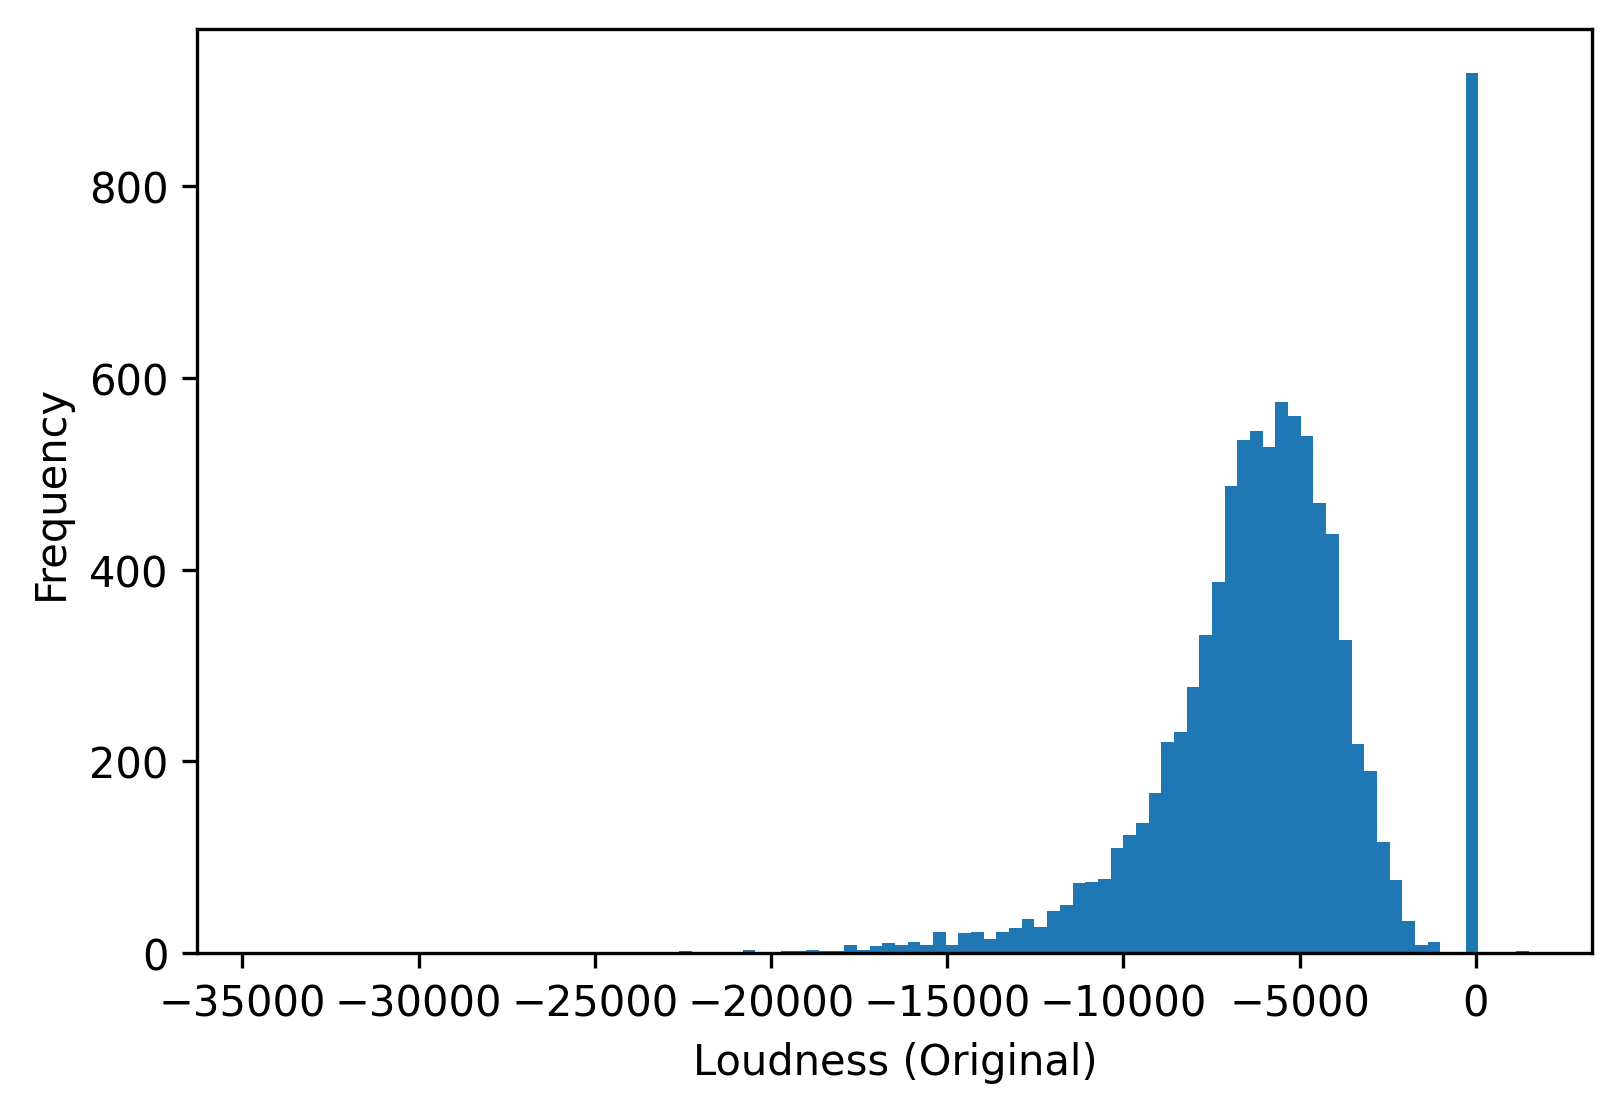
\includegraphics[width=0.85\textwidth]{images/loudness_histogram_original.png}
  \caption{Original loudness distribution showing extreme outliers and irregular scaling.}
  \label{fig:appendix_loudness_original}
\end{figure}

\begin{figure}[H]
  \centering
  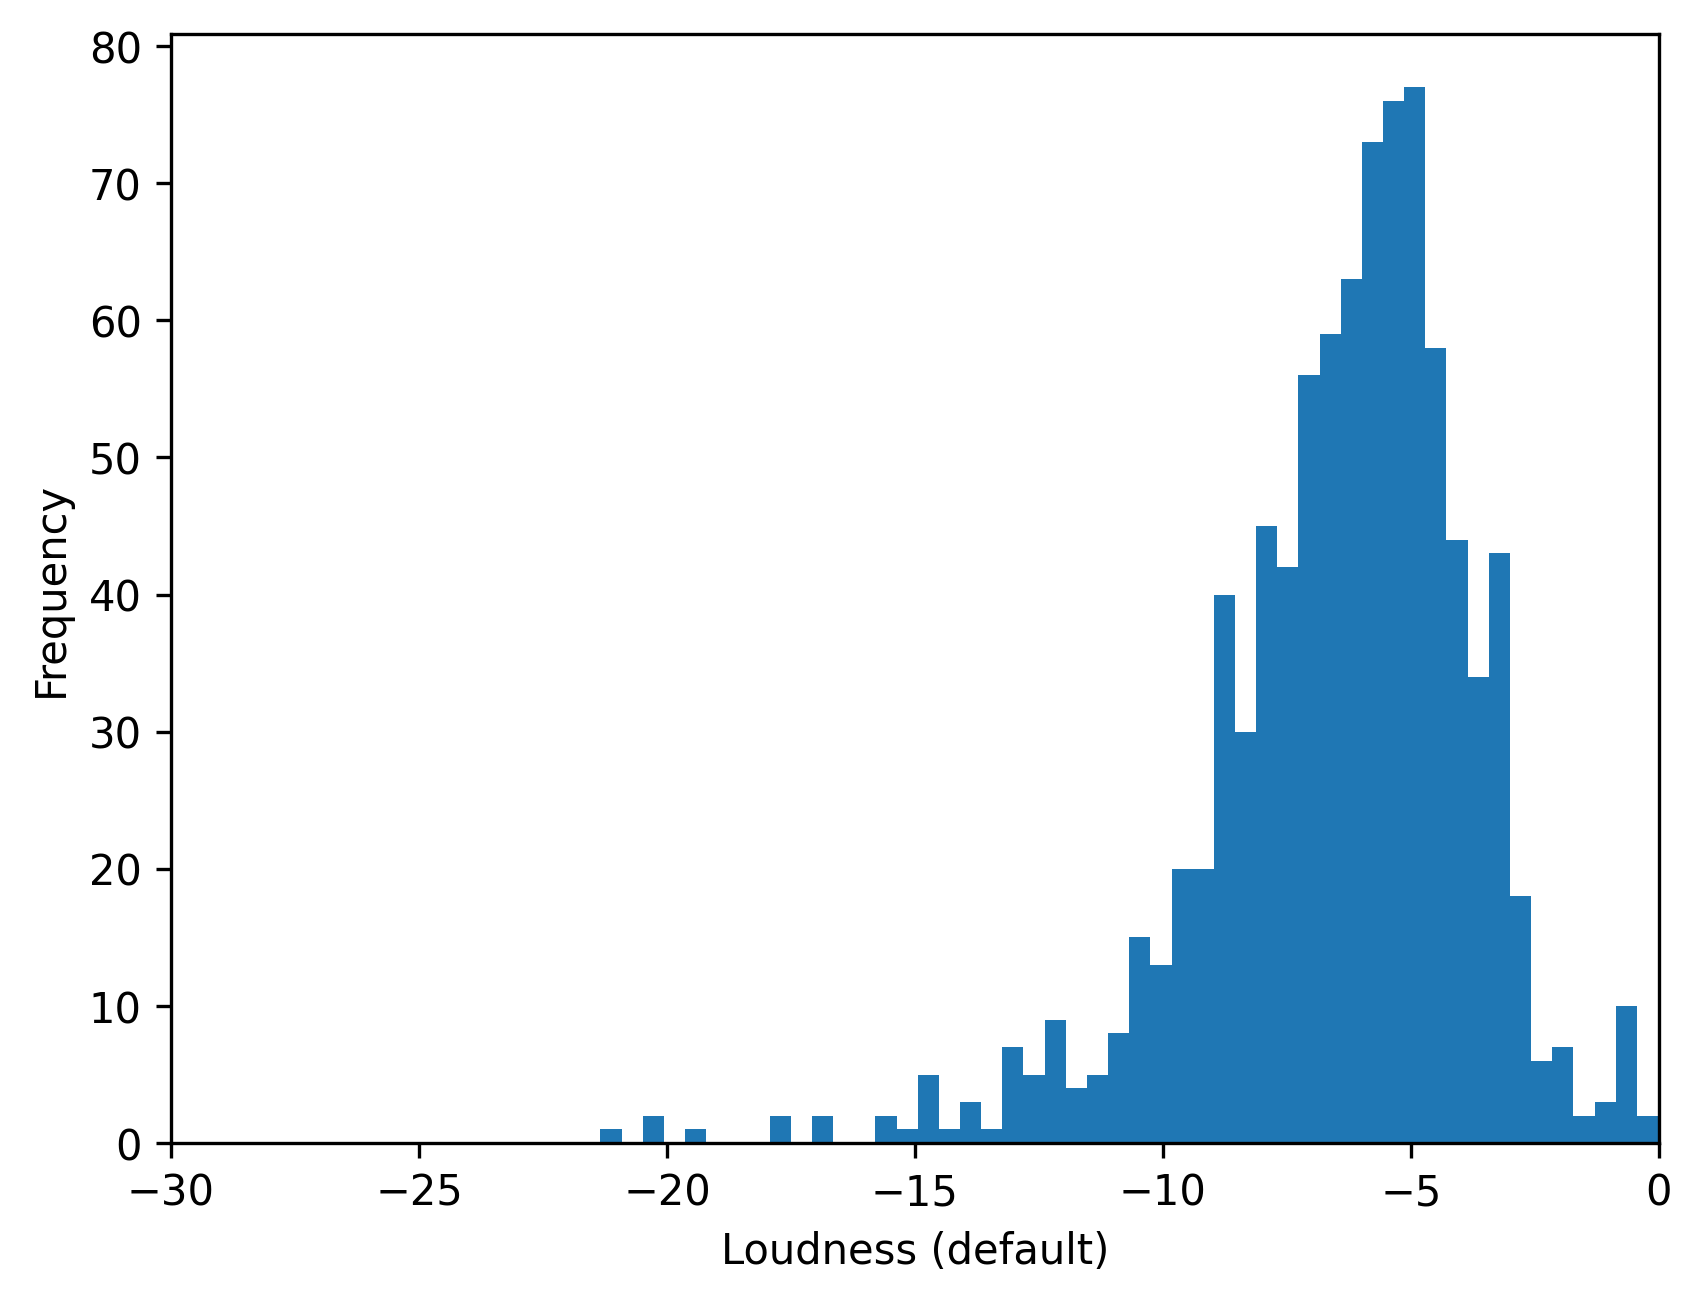
\includegraphics[width=0.85\textwidth]{images/loudness_histogram_clipped.png}
  \caption{Distribution after clipping to realistic digital audio levels (–22\,dB to –2.5\,dB).}
  \label{fig:appendix_loudness_clipped}
\end{figure}

\begin{figure}[H]
  \centering
  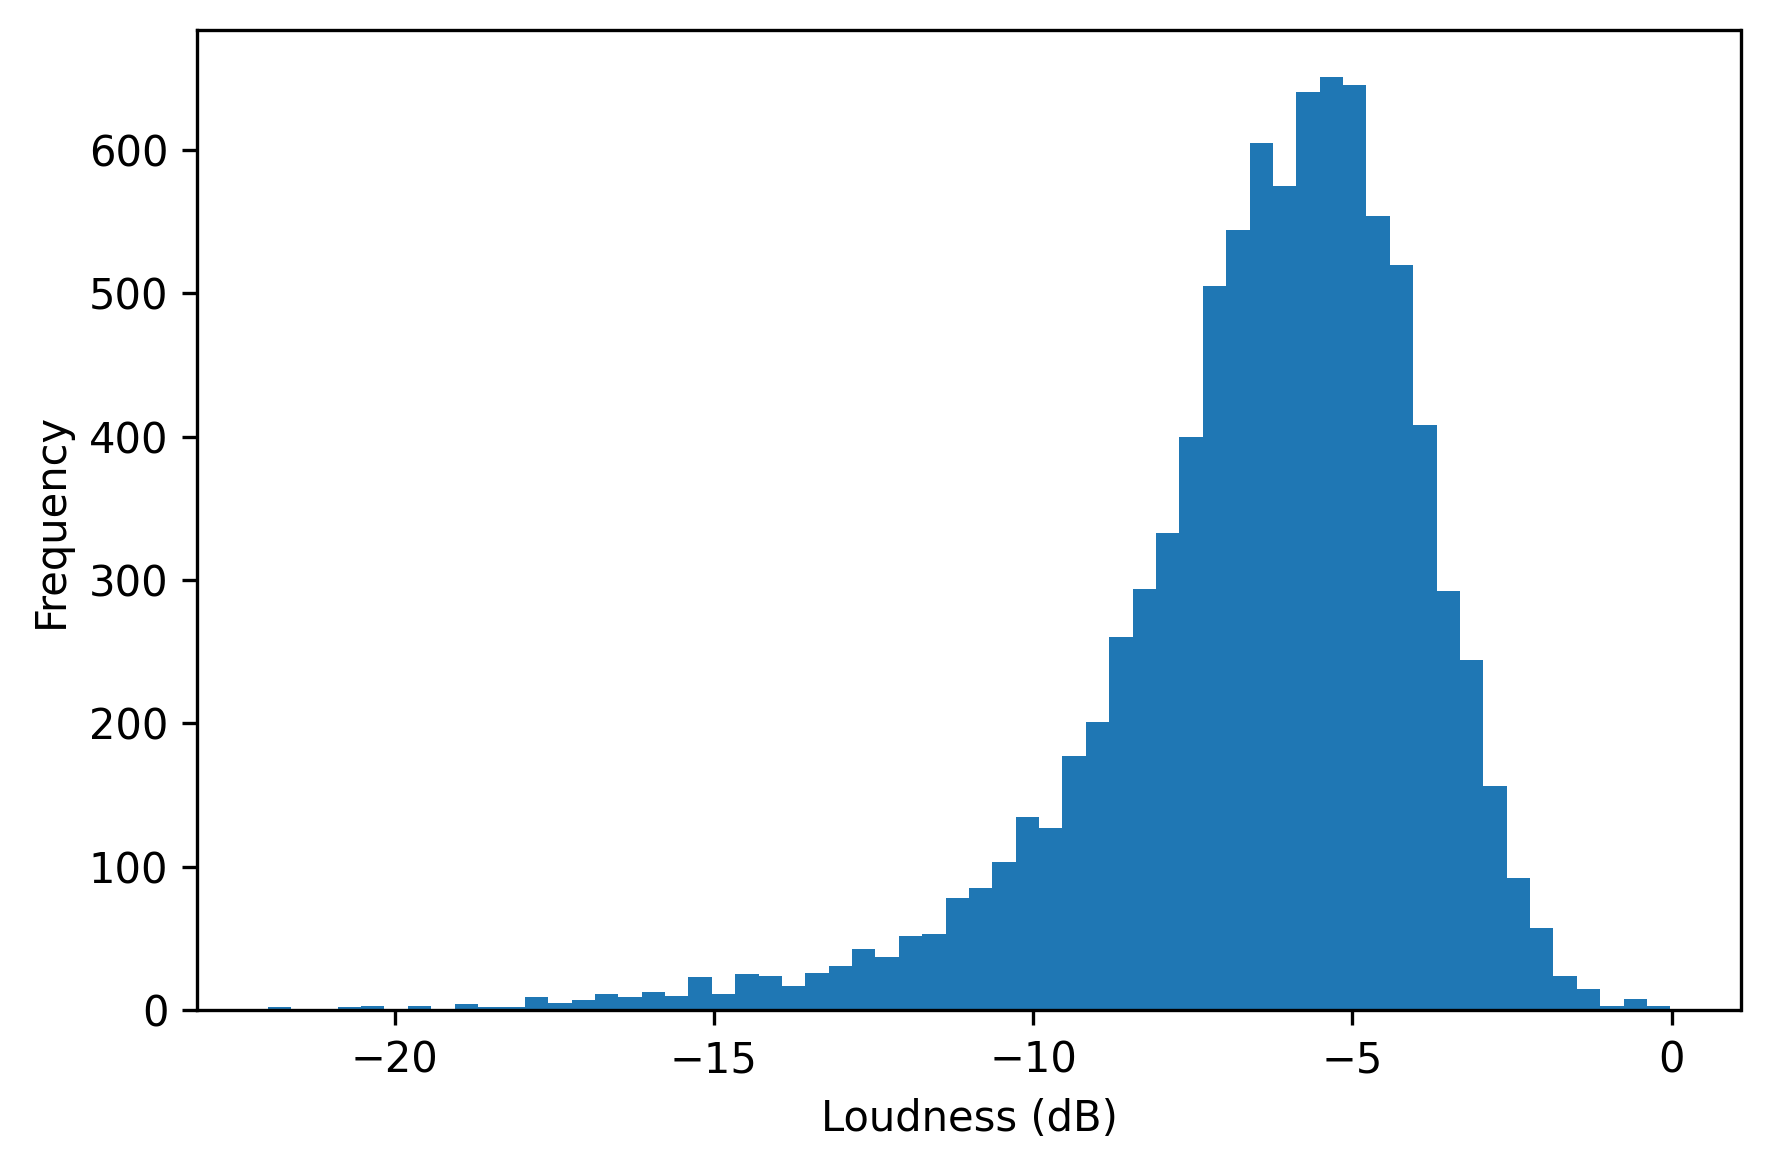
\includegraphics[width=0.85\textwidth]{images/loudness_histogram_scaled.png}
  \caption{`Zoomed in' Original Loudness values within typical range }
  \label{fig:appendix_loudness_scaled}
\end{figure}

\newpage
\section{Genre Classifications}\label{appendix:genre-classifications}

\begin{table}[h]
\centering
\caption{Results for different max\_iter values}
\label{tab:max_iter_results}
\begin{tabular}{cccccccc}
\hline
max\_iter & 600 & 700 & 800 & \textbf{900} & 1000 & 1500 & 2000 \\
\hline
auc & 0.854 & 0.854 & 0.854 & \textbf{0.855} & 0.855 & 0.855 & 0.855 \\
\hline
\end{tabular}
\end{table}

\begin{table}[h]
\centering
\caption{AUC values for different max\_depth and min\_samples\_leaf combinations}
\label{tab:hyperparameter_tuning}
\begin{tabular}{l|cccccc}
\hline
 & \multicolumn{6}{c}{\textbf{max\_depth}} \\
\cline{2-7}
\textbf{min\_samples\_leaf} & {5} & \textbf{7} & {10} & {12} & {15} & {17} \\
\hline
1  & 0.819 & 0.823 & 0.792 & 0.781 & 0.760 & 0.751 \\
5  & 0.803 & 0.827 & 0.826 & 0.812 & 0.806 & 0.805 \\
10 & 0.803 & 0.823 & 0.825 & 0.825 & 0.823 & 0.817 \\
15 & 0.818 & 0.850 & 0.858 & 0.855 & 0.855 & 0.855 \\
\textbf{20} & 0.817 & \textbf{0.859} & 0.850 & 0.850 & 0.846 & 0.846 \\
100 & 0.829 & 0.847 & 0.846 & 0.846 & 0.846 & 0.846 \\
200 & 0.800 & 0.800 & 0.800 & 0.800 & 0.800 & 0.800 \\
500 & 0.773 & 0.773 & 0.773 & 0.773 & 0.773 & 0.773 \\
\hline
\end{tabular}
\end{table}

\begin{figure}[h]
\centering
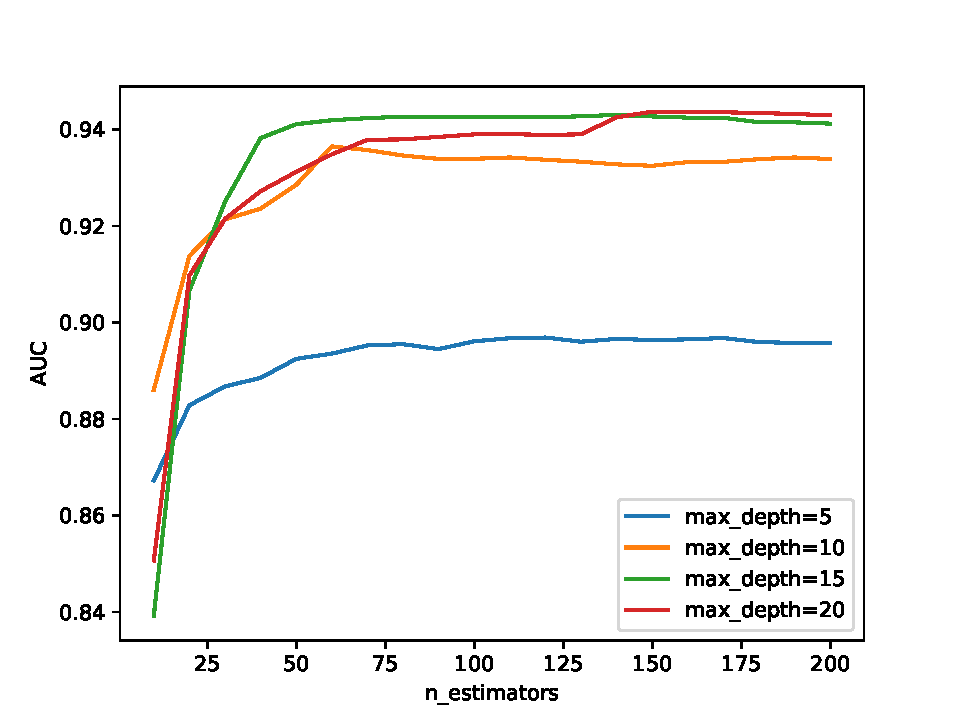
\includegraphics[width=0.8\textwidth]{images/max_depth.pdf}
\caption{AUC Values for different n\_estimators and min\_samples\_leaf combinations}
\label{fig:max_depth}
\end{figure}

\begin{figure}[h]
\centering
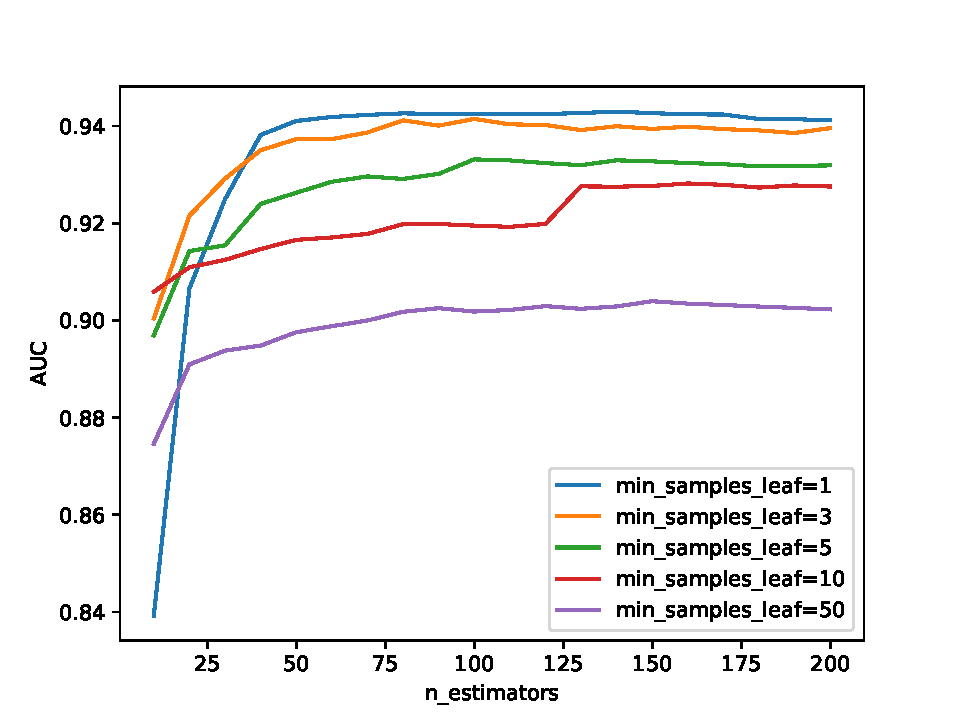
\includegraphics[width=0.8\textwidth]{images/min_samples_leaf.pdf}
\caption{AUC Values for different n\_estimators and min\_samples\_leaf combinations}
\label{fig:min_samples_leaf}
\end{figure}

\begin{figure}[h]
\centering
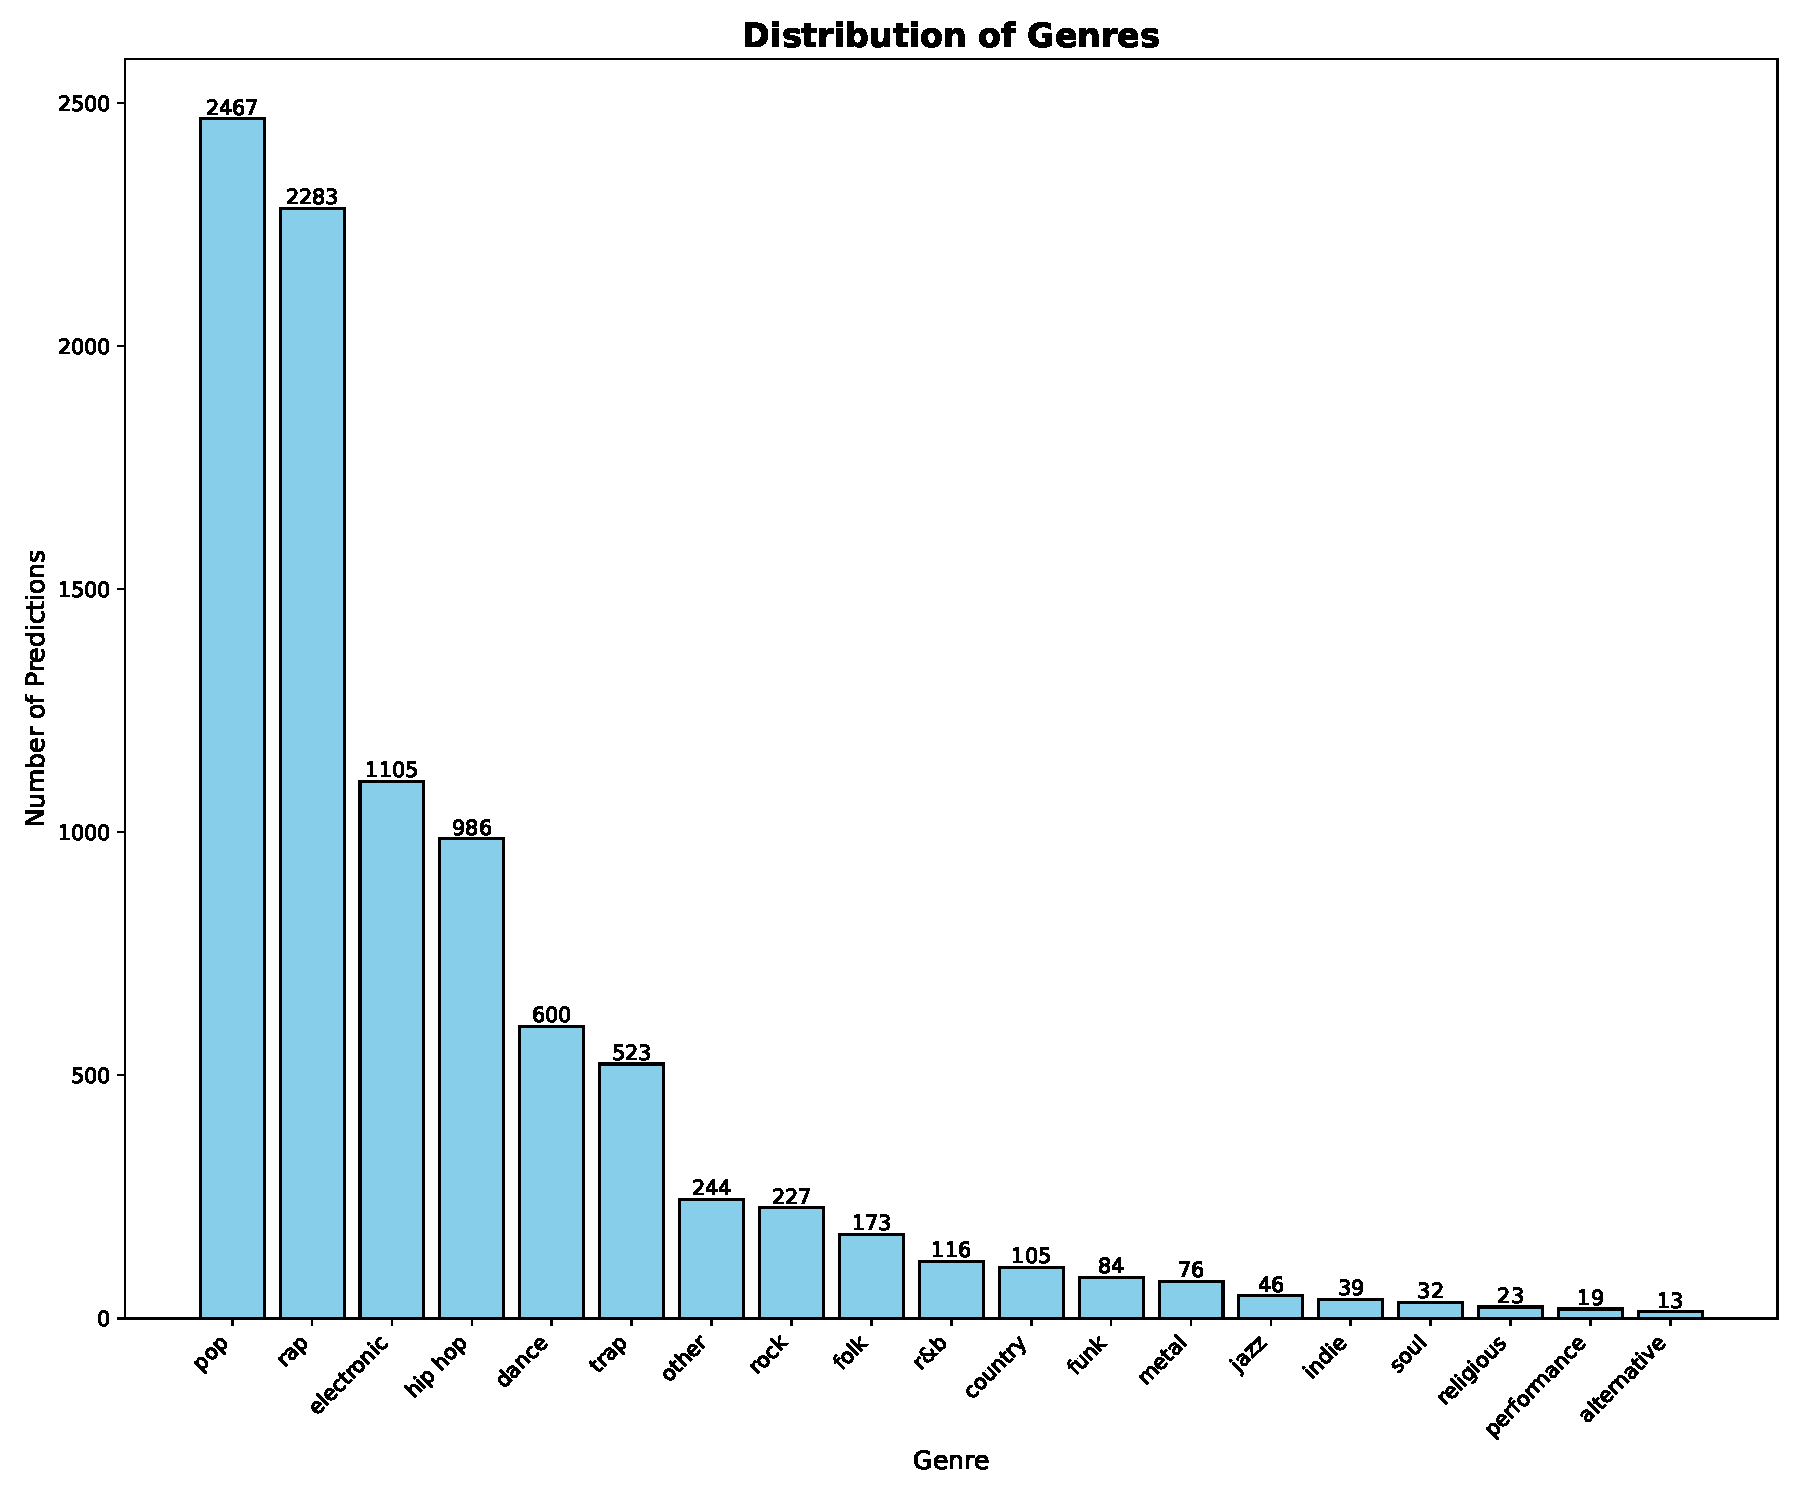
\includegraphics[width=0.8\textwidth]{images/complete_genre_distribution.pdf}
\caption{Genre Distribution of Originally Labelled Songs}
\label{fig:complete_genre_distribution}
\end{figure}

\begin{figure}[H]
\centering
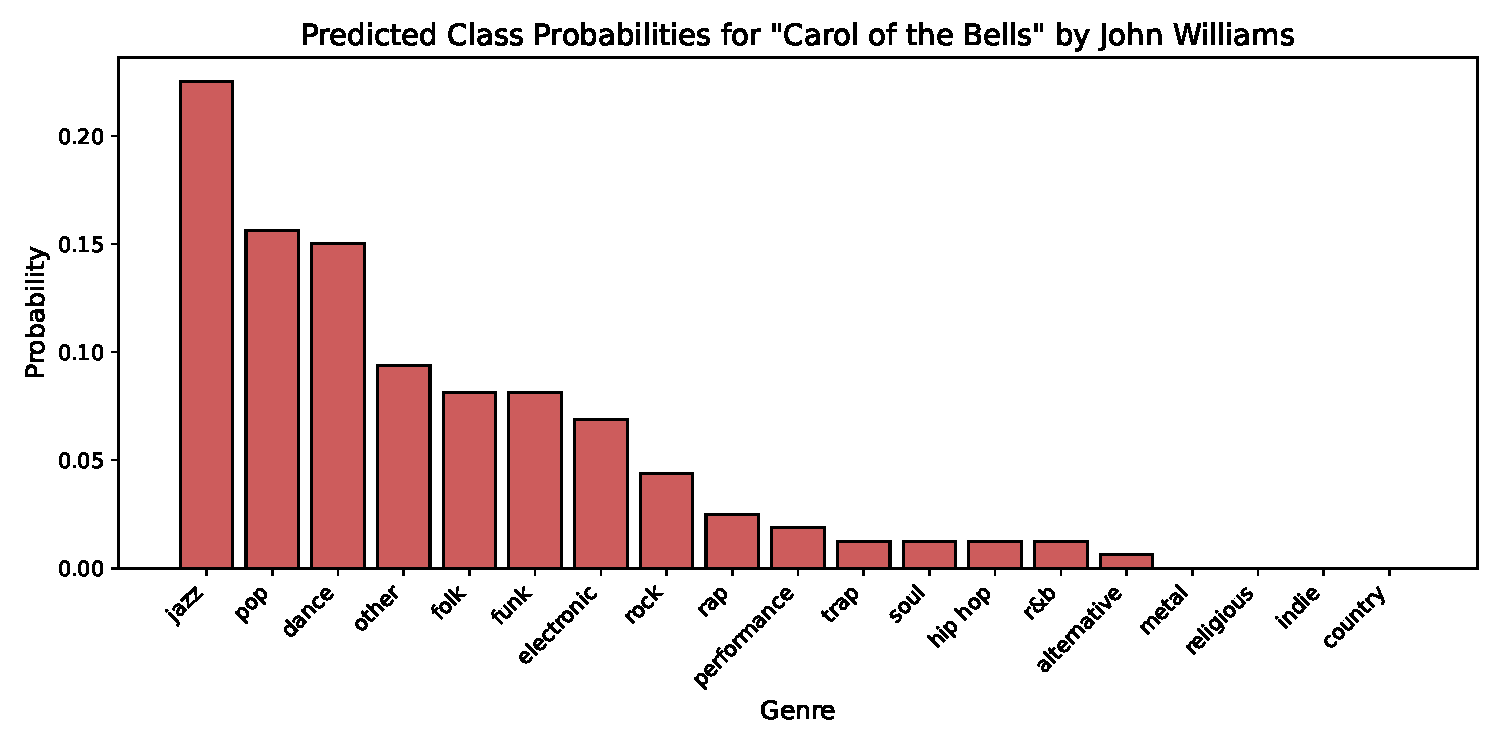
\includegraphics[width=0.8\linewidth]{images/carol_of_the_bells_genre_probs.pdf}
\caption{Predicted genre for `Carol of the Bells' by Random Forest}
\label{fig:carol}
\end{figure}

\begin{table}[h]
\centering
\begin{tabular}{|l|l|}
\hline
\textbf{Hyperparameter} & \textbf{Value} \\
\hline
Input layer neurons & 128 \\
Hidden layers neurons & 64, 32 \\
Hidden layer activation & ReLU \\
Dropout & Yes \\
Output layer neurons & 19 (softmax) \\
Loss function & Categorical cross-entropy \\
Optimiser & Adam \\
Learning rate & $1.5\times10^{-4}$ \\
Batch size & 64 \\
Epochs & 200 \\
Early stopping & On validation loss \\
Learning rate reduction & Yes \\
Evaluation metric & ROC-AUC \\
Test set ROC-AUC & 0.898 \\
\hline
\end{tabular}
\caption{Hyperparameters for the multi-layer feedforward neural net}
\label{tab:hyperparam}
\end{table}

\newpage
\section{Sample Recommendations}\label{appendix:recommendations}
Tables displaying the top 20 song recommendations by the semantic model with the random forest genres for a sample of songs selected for being the highest ranked song in their respective genre.

\begin{table}[H]
\centering
\tiny
\begin{tabular}{lll|ccc}
Title & Primary Artists & Genre & Feature Sim. & Lyric Sim. & Weighted Score \\
\hline
more than life (feat. glaive) & machine gun kelly & electronic & 0.977392 & 0.566658 & 0.689878 \\
when i'm alone & post malone & pop & 0.800297 & 0.631404 & 0.682072 \\
bloody valentine & machine gun kelly & rock & 0.881019 & 0.587870 & 0.675814 \\
pill breaker (feat. blackbear \& machine gun kelly) & travis barker, trippie redd & rap & 0.939686 & 0.552461 & 0.668628 \\
escapism. & 070 shake, raye & rap & 0.929992 & 0.551707 & 0.665192 \\
lovers rock & tv girl & pop & 0.758086 & 0.618917 & 0.660668 \\
me \& you together song & the 1975 & rock & 0.912087 & 0.551254 & 0.659504 \\
everlong & foo fighters & rock & 0.975724 & 0.521415 & 0.657707 \\
escapism. - sped up & 070 shake, raye & rap & 0.881554 & 0.553867 & 0.652173 \\
t r a n s p a r e n t s o u l (feat. travis barker) & willow & electronic & 0.987203 & 0.507923 & 0.651707 \\
numb & linkin park & metal & 0.939851 & 0.527606 & 0.651280 \\
awful things & lil peep & rap & 0.973393 & 0.511724 & 0.650224 \\
sex with my ex & lil peep & rap & 0.891393 & 0.543637 & 0.647964 \\
too much (feat. timbaland) & zayn & electronic & 0.827619 & 0.569812 & 0.647154 \\
today was a fairytale (taylor's version) & taylor swift & pop & 0.955472 & 0.513369 & 0.646000 \\
addicted to you & avicii & electronic & 0.863271 & 0.551199 & 0.644821 \\
bad lil vibe (feat. jeremih) & ksi & electronic & 0.742938 & 0.600327 & 0.643111 \\
i would like & zara larsson & pop & 0.885147 & 0.538640 & 0.642592 \\
the kind of love we make & luke combs & country & 0.698897 & 0.616537 & 0.641245 \\
in my feelings & lana del rey & rap & 0.795368 & 0.571135 & 0.638405 \\
\end{tabular}
\vspace{0.5em}
\caption{Recommendations for `Mr. Brightside' by The Killers, \texttt{genre == 'alternative'}}
\end{table}

\begin{table}[H]
\centering
\tiny
\begin{tabular}{lll|ccc}
Title & Primary Artists & Genre & Feature Sim. & Lyric Sim. & Weighted Score \\
\hline
chrome heart tags & lil uzi vert & rap & 0.929842 & 0.613738 & 0.708569 \\
dancing feet (feat. dnce) & kygo & electronic & 0.839625 & 0.633678 & 0.695462 \\
oh caroline & the 1975 & folk & 0.859839 & 0.608959 & 0.684223 \\
more than my hometown & morgan wallen & country & 0.856835 & 0.600109 & 0.677127 \\
had enough (feat. quavo \& offset) & don toliver & electronic & 0.884177 & 0.584690 & 0.674536 \\
ruin my life & zara larsson & pop & 0.879575 & 0.581627 & 0.671012 \\
skrt on me (feat. nicki minaj) & calvin harris & electronic & 0.764107 & 0.623839 & 0.665920 \\
i feel it coming & daft punk, the weeknd & pop & 0.914914 & 0.559155 & 0.665883 \\
every summertime & niki & r\&b & 0.777917 & 0.614114 & 0.663255 \\
the way life goes (feat. oh wonder) & lil uzi vert & rap & 0.940556 & 0.542122 & 0.661652 \\
love lost & mac miller, the temper trap & rap & 0.921352 & 0.550048 & 0.661439 \\
one touch & jax jones, jess glynne & trap & 0.797045 & 0.597128 & 0.657103 \\
die 4 me & halsey & electronic & 0.905305 & 0.549991 & 0.656585 \\
shivers & ed sheeran & pop & 0.868952 & 0.564877 & 0.656099 \\
to the bone & pamungkas & indie & 0.776714 & 0.598403 & 0.651896 \\
paradise & george ezra & dance & 0.766078 & 0.601563 & 0.650917 \\
je me casse & destiny & dance & 0.745411 & 0.607984 & 0.649212 \\
stay (don't go away) [feat. raye] & david guetta & electronic & 0.772224 & 0.592332 & 0.646299 \\
moonlight sunrise & twice & pop & 0.912550 & 0.532135 & 0.646259 \\
shape of you & ed sheeran & pop & 0.837973 & 0.560446 & 0.643704 \\
\end{tabular}
\vspace{0.5em}
\caption{Recommendations for `Positions' by Ariana Grande, \texttt{genre == 'pop'}}
\end{table}

\begin{table}[H]
\centering
\tiny
\begin{tabular}{lll|ccc}
Title & Primary Artists & Genre & Feature Sim. & Lyric Sim. & Weighted Score \\
\hline
caroling, caroling & nat king cole & jazz & 0.634603 & 0.711048 & 0.688114 \\
jingle bells (feat. the puppini sisters) & michael bublé & other & 0.679108 & 0.650798 & 0.659291 \\
silver bells & dean martin & jazz & 0.580072 & 0.686986 & 0.654912 \\
the man with the bag & kay starr & other & 0.845278 & 0.545336 & 0.635318 \\
silver bells & bing crosby, carol richards & other & 0.523662 & 0.673061 & 0.628241 \\
rockin' around the christmas tree & brenda lee & other & 0.682957 & 0.568862 & 0.603090 \\
white christmas & michael bublé & other & 0.904983 & 0.472653 & 0.602352 \\
it's beginning to look a lot like christmas & bing crosby & other & 0.796511 & 0.516297 & 0.600361 \\
holly jolly christmas & michael bublé & other & 0.737786 & 0.530685 & 0.592816 \\
sleigh ride & ella fitzgerald & jazz & 0.594610 & 0.590538 & 0.591760 \\
let it snow! - 10th anniversary & michael bublé & other & 0.909147 & 0.449577 & 0.587448 \\
man with the bag & jessie j & pop & 0.686366 & 0.538425 & 0.582807 \\
a holly jolly christmas & brett eldredge & country & 0.660252 & 0.548635 & 0.582120 \\
winter wonderland & tony bennett & jazz & 0.721307 & 0.516535 & 0.577966 \\
cool yule & louis armstrong, the commanders & jazz & 0.759679 & 0.497927 & 0.576453 \\
here comes santa claus (right down santa claus lane) & elvis presley & rock & 0.441543 & 0.631554 & 0.574550 \\
it's the most wonderful time of the year & andy williams & other & 0.638231 & 0.544871 & 0.572879 \\
have yourself a merry little christmas (feat. esperanza spalding) & john legend & pop & 0.596991 & 0.553322 & 0.566423 \\
it's beginning to look a lot like christmas & michael bublé & other & 0.654717 & 0.525723 & 0.564421 \\
jingle bell rock & bobby helms & other & 0.632789 & 0.534558 & 0.564028 \\
\end{tabular}
\vspace{0.5em}
\caption{Recommendations for `Carol of the Bells' by John Williams, \texttt{genre == 'performance'}}
\label{tab:carol-of-the-bells}
\end{table}

\end{document}

%%% Local Variables:
%%% mode: latex
%%% TeX-master: t
%%% End:


\iffalse
\section{(temp) Current Progress}
\begin{itemize}
    \item Data cleaning and normalisation
    \begin{itemize}
        \item Parsed out primary vs feature artists from titles via regex pattern matching
        \item Created new `Primary Artist' and `Featuring Artist' features
        \item Created helper datasets: 
        \begin{itemize}
            \item Unique Artist , including mean feature values
            \item Unique Songs dataset
            \item Temporal dataset with new primary/featuring artist features
        \end{itemize}
        \item Rescaled `Loudness' Feature
        \item Noticed all instances of `na' had been removed from the data set. For example, there is an entry for `il tech' as a song by Jack Harlow, which corresponds to the true song `Nail tech'
    \end{itemize}
    \item Feature Engineering/Addition
    \begin{itemize}
        \item \textbf{Lyrics and language information}: used Genius API, and lingua-py to analyse language. Had to manually correct about 30 misclassification's
        \item \textbf{Retrieved additional spotify metrics}: including track popularity, artist followers, artist popularity, artist genres, and explicit flag for tracks
        \item \textbf{One-hot encoded nationality, continent, languages}: for use with PCA
        \item \textbf{Genre Processing:} Created `super-genre' categories 
        \item \textbf{Artist Profile generation} We built artist profiles with per metrics means and standard deviations for the 7 given audio features, for use in artist prediction
    \end{itemize}
    \item Exploratory Data Analysis
    \begin{itemize}
        \item \textbf{Correlation analysis of original features:} discovered no surprising correlations within data
        \item \textbf{Genre Distributions:} 
        \begin{itemize}
            \item By retrieving artist genres from spotify API, we find distribution of genres over the entire dataset.
            \item Due to a bug with the Spotify API, not all artists return a genre
            \item Songs with no genre (due to no artist genre) = 3890
            \item Songs with multiple genres = 2425
            \item Songs with a single genre = 2846
        \end{itemize}
        
        \item \textbf{Lyrical Analysis:} Performed basic NLP tasks on track lyrics to foster analysis of lyrics and how they may tie in to rankings and preference
        \item \textbf{PCA}: Performed initial PCA on track features, and one hot encoded nationality/continent/language/explicit. Concerned not enough features for PCA to be of use.
    \end{itemize}
    \item Modelling/Experimentation
    \begin{itemize}
        \item \textbf{Guess the Artist, given a song}
        \begin{itemize}
            \item We model each artist's music as a Gaussian Distribution over their song metrics
            \item We then compute how likely a given song is to be by an artist (via likelihoods)
            
        \end{itemize}
        \item \textbf{Feature-based track recommender:} using track features, built basic song recommender, given a song, which suggests similar songs. Used cosine similarity as metric
        \item \textbf{Hybrid feature + lyric vs. TF-IDF recommender:} Built upon previous recommender with semantic analysis and TF-IDF. Compared TF-IDF only vs. semantic only vs. hybrid vs. features only vs. random recommendations via silhouette score (cluster overlap), avg. recommendation consistency (feature similarity between recommendations and the query), artist coherence score (clustering within artist discography), avg. pairwise distance and embedding efficiency.
        \item \textbf{Genre semantic clustering:} 
        \begin{itemize}
            \item Explored both k-means and agglomerative clustering on genre text embeddings. Limited relevant results, which motivated our curation of `super-genres'
            \item \textit{Method:} extract artist genres from track, if multiple, assign individual genres to super-class, then take most common superclass as the track superclass
            \item E.g: the song dákiti by bad bunny and jhayco, has these genres attached:  reggaeton, trap latino, urbano latino, latin. Reggaeton is electronic, trap latino is trap, urbano latino is dance, latin is dance. Thus, the overall genre of the song is dance.
        \end{itemize}
    \end{itemize}
    \item Finalise supplementary task
\end{itemize}

\section{(temp) Plans for completion}

\begin{enumerate}
    \item Refactor and clean code base, aggregate datasets
    \item \underline{Primary Task: Genre super-class prediction}:
    \begin{itemize}
        \item Finish super-genre mapping 
        \item Decide on models on to perform genre prediction (randomforest, log reg, non-linear methods)
        \item Determine metrics: precision, F1, accuracy, means/std
        \item error analysis
    \end{itemize}
    \item \underline{Secondary task: Track recommender} 
    \item Consider tasks using temporal patterns and rank, or collaborations
    \item Writing
    \begin{itemize}
        \item Populate introduction, background
    \end{itemize}
\end{enumerate}
\fi